\documentclass[acmsmall,screen,review]{acmart}
\input{glyphtounicode}
\pdfgentounicode=1
\usepackage{tabularx}
\usepackage{xltabular}
\usepackage{longtable}
\usepackage{graphicx}
\usepackage{booktabs}
\usepackage{ragged2e}
\newcolumntype{Y}{>{\RaggedRight\arraybackslash}X}
\newcolumntype{Z}{>{\RaggedLeft\arraybackslash}X}
\settopmatter{printacmref=false}
\setcopyright{none}
\acmJournal{TQC}
\acmYear{2026}
\begin{document}

\title{A Verifiable and Cost-Controlled Experiment Platform for Cloud Quantum Optimization Benchmarks}
\author{Hiroaki Tobita}
\affiliation{\institution{Advanced Institute of Industrial Technology}\city{Tokyo}\country{Japan}}
\email{tobita-hiroaki@aiit.ac.jp}
\begin{abstract}
A cloud quantum optimization benchmark can produce an internally consistent record from an input that its published statistics no longer describe, and can be charged for circuits nobody asked it to run. Both happened to the study behind this paper. The platform built in response binds the pinned statistics, the enumerated references, the run table and the per-run artifacts through thirteen checked relations, refuses the expensive configurations before submission, and measures what reconstruction costs; each part is evaluated against a control that keeps the practice it replaces. What a check can settle is bounded by the record it reads. Expectations over the run table, stated as a pandera schema, detect eight of ten injected faults and nearly as many of the random mutations that change a reported number as the thirteen relations do; over every mutation of the table the relations detect about twice as many, mostly through identities the schema did not state, and mutations confined to the pinned inputs or the per-run artifacts are caught only by relations that read those files --- on the main record and on two sibling records. A block re-run from a statistic perturbed by a tenth keeps the table consistent, moves reported numbers, and passes every expectation; catching it took a cross-record check that the aggregation gate, as first released, did not run; it runs it now. On the service, one sampling call left trainable created 177 tasks where a frozen one creates one; the provider's dollar cap excludes the simulator where that happened, and its cost-control sample, deployed as documented, metered nothing while 400 tasks ran and, corrected, let a median of 47 tasks past the limit. What each of three reconstruction levels costs is measured.
\end{abstract}
\ccsdesc[500]{Software and its engineering~Software verification and validation}
\ccsdesc[300]{Hardware~Quantum computation}
\ccsdesc[300]{Information systems~Data provenance}
\ccsdesc[300]{General and reference~Experimentation}

\keywords{reproducibility; experiment management; data provenance; quantum cloud services; QAOA; cost control; fault injection; software engineering for quantum computing}
\maketitle



\section{Introduction}

A cloud quantum optimization benchmark depends on more than its algorithm. It depends on the input values the provider returned when it was run, on the circuits the client library decided to execute, and on the agreement of the records the analysis reads. At each of those three an experiment script tends to write down what it assumed rather than what happened --- an inference where a fact belongs --- and this paper is about designing the platform so that it writes the fact. The platform is therefore built for the run that goes wrong: every mechanism of Section 3 is the fixed form of a failure this project met (Tables 13 and 14), and the evaluation consists of making it fail on purpose.


A benchmark of a variational quantum algorithm on a cloud service is an experiment with three moving parts that an experiment script tends to treat as fixed. The \textit{input} is not a fixed dataset but a query --- in the finance setting, adjusted closing prices that the provider revises between calls, so that two runs over the same date window need not be the same problem. The \textit{execution} is metered by the task and the shot, and the number of tasks is decided not by the algorithm's description but by the framework's choice of differentiation method, which it makes from the trainability flag of a tensor and not from whether anyone asked for a gradient. The \textit{record} is large --- thousands of runs, each with angles, a state, a shot batch and a bill --- and a mix-up between any two of its parts (a row pasted from a different window, a batch drawn from the wrong state, a column dropped by a writer that takes its header from the first row) leaves the aggregate looking plausible.


At each of the three the record holds an inference: a date range stands in for the values it retrieved; the algorithm's description stands in for the circuits the service executed; a printed ``done'' stands in for how a job ended; a plausible aggregate stands in for the agreement of the records beneath it. The numerical study this platform served \cite{ref1} recorded 2,565 QAOA runs across three problem sizes, thirty instances, five seeds and six penalty settings, with 900 further runs that move the constraint out of the cost and into the ansatz (the parametrized circuit) and control arms on a cloud simulator and a trapped-ion device. It met seven implementation defects, five of which changed reported numbers (Section 6, Table 13), and two further incidents that concerned the record's inputs and its bill rather than a run. Every one of the nine had the same shape: a window pinned by date that the provider revised underneath; a sampling call billed as 177 tasks because the framework, not the algorithm, decided the count; a ``shot-seed control'' that re-seeded a generator the device did not read; a device's answer replaced by a client library's misparse of it; a batch drawn from the initial state while the record said the final one. Eight of the nine were found by inspection or by an ad hoc comparison and the last by a check between two records that should have agreed and did not (Section 6): detection depended on luck, because the inference was never written down as something that could be checked.


The present paper asks how the experiment platform should be designed so that the inference is replaced by a record at each of the three places, and the records are checked against one another by a machine --- so that mix-ups are detected, unintended billable execution is refused before submission, and a third party can rebuild the results at a known cost. It answers with three design principles, one per place, each stated with what it does and does not prevent, and each evaluated against a control configuration that keeps the inference. The principles live in the experiment platform's own code and records, not in the cloud provider's settings: no provider setting binds a run to its market statistics, checks a batch against its state, or records how a job ended, and the one provider control that bears on billing --- a per-device dollar cap --- enters the evaluation as a \textit{control} for the second principle, not as its implementation. The platform is one Python package --- the solver and its guards, the experiment drivers, the record's thirteen checks and the three harnesses that evaluate them --- published at \texttt{github.\allowbreak{}com/\allowbreak{}tobita\allowbreak{}Q/\allowbreak{}qaoa-\allowbreak{}portfolio-\allowbreak{}penalty-\allowbreak{}benchmark} (release \texttt{v1.3}; the release E-S3 reconstructs at three levels is \texttt{v1.2}, doi:10.5281/zenodo.24032941); the Availability section lists what is in it and what is not. The setting is deliberately small: one researcher, one GPU workstation, a commercial cloud account, and a total cloud bill of \$42.59 for the two papers' runs. Systems reported from dedicated quantum infrastructure with a team behind them can be read but not repeated by most of their readers; the unit of reproduction here is one person with one machine and a credit card. The machine is a laptop for the first reconstruction level of Section 3.3 and a CPU for the second, which take seconds and minutes; only the third asks for the GPU hours the cross experiment --- the numerical study's full factorial sweep, E1 --- cost.


\textbf{P1 --- Bind each record to its inputs and its outputs, and make the relations between records checkable.} A run row carries the instance's input digest, the penalty constant and its label, the initial angles, the final angles, the exact-state quantities, the shot summary and the cost; a per-run artifact carries the trajectory, the stored probabilities and the shot counts; a reference row per instance carries the enumerated optimum and the penalty scales; the derived statistics are the pinned input. Thirteen checks connect these records: consistency conditions that a correct record satisfies, numerical recomputations within stated tolerances, and a few diagnostics that mark a run to look at. A fault appears as a check that reports.


\textbf{P2 --- Refuse billing by configuration, before submission.} A quantum processing unit (QPU) cannot be named as the optimizer's backend: the constructor refuses it before any cloud object exists and the command-line driver refuses it before constructing a solver. The final sampling call receives frozen angles, so that the framework's fallback from adjoint differentiation, which a simulator computes in one pass, to parameter-shift differentiation, which evaluates the circuit twice per parameter and multiplies the tasks of one sampling call by the number of parameters --- cannot occur. A cloud run must name itself and cannot overwrite the committed baseline. A dollar cap is layered on top, not relied on.


\textbf{P3 --- Offer reconstruction at three levels and record what each one cost.} Tables and figures from committed aggregates (seconds); one instance end to end (minutes on a CPU); the cross experiment from its manifest (GPU hours). What bounds the loss when a long run is interrupted, and what the job writes down about how it ended rather than leaving it to be inferred, is Section 3.3.


Each principle is stated with what it prevents and what it does not (Section 3), and each is evaluated against a control (Section 4): the record with its verification relations against a schema-only pipeline (E-S1, fault injection); the structural guards against no guard and against a spending limit alone (E-S2, guard-stage measurement on a stand-in device); the reconstruction levels against the same package without its derived statistics and without its per-run artifacts, and against what a restart would have redone (E-S3, a clean-room clone; Section 4.3). The evaluation touches the cloud account only to observe two facts on SV1, the provider's managed state-vector simulator, that the guard harness had modelled, and to measure an account-level cost control over six runs (1,249 tasks, \$4.69 in all; Section 5.2, Table~S3 of the supplement).


\textbf{What form these problems take in a quantum experiment.} None of what this platform binds is unique to quantum computing: an input the provider revises, a job whose end state is inferred, a metered call whose cost the framework decides, a result that is a sample, a package a reader has to rebuild. What is worth stating is the shape each takes here, because the shape is what the design answers. The billable unit is decided by the trainability of a tensor, because a gradient of a quantum circuit \textit{is} more circuits: one optimizer step on a device without adjoint support executes 1 + 2p$\cdot$[C(N,2) + 2N] tasks, so a flag in the client library moves the bill by two orders of magnitude. A result is a sample, and on a simulator the distribution behind it is computable and was stored, so a shot count can be tested against the record itself rather than against a model of it --- on hardware the same test has no force, because a mismatch is as likely to be noise (Section 2.1 says what is and is not new about that). Three more, none of them quantum in themselves: the provider's dollar cap exists for hardware and not for the simulator on which this project's real fallback occurred; the device this paper needed answered \texttt{OFFLINE} to 336 queries over seven days, so a hardware observation is a waiting problem; and single-precision state quantities are not portable across hosts, so the README must say in advance which columns a reader should expect to move. A provider's policy, a queue and a floating-point fact --- recognisable anywhere, and each with a particular edge here.


\textbf{Contributions.} The first is a result about verification, the second is two measurements of a metered stack, and the third is a costed report; each names the sections that state it and evidence it.


\begin{enumerate}
\item \textbf{A verification specification for a QAOA benchmark record, and how far it reaches.} Thirteen relations bind the pinned inputs, the enumerated references, the run rows and the per-run artifacts of a metered run, each stated with what it reads and what kind of rule it is (Section 3.1). Fault injection on a 2,565-run record and on two sibling records measures what they detect against a schema-only pipeline and against the same declarative control stated as a pandera schema, separates the mutations that change a reported number from the other inconsistencies, and counts the increment that each kind of record read brings (Section 5.1, Tables 3--6). One relation compares a shot batch with the probability the simulator computed for the recorded state, by an exact binomial tail with a stated false-alarm bound; it reads run-row columns, and what this paper supplies is the comparison and its calibration, not a capability a validation library lacks.
\item \textbf{What a metered stack actually bills and actually refuses.} The circuits one optimizer step sends on a device that offers no derivative method --- 177 / 361 / 609 / 921 at N = 8 / 12 / 16 / 20, each billed as one task, with the fallback re-observed on the service (Sections 3.2, 5.2) --- and the provider's cost controls measured rather than assumed: a per-device dollar cap that does not exist for simulators, and an account-level sample that, deployed as its documentation says, metered nothing while 400 tasks passed and, after three changes, let a median of 47 tasks past its limit over five repetitions (Table 9). We have not found either reported, and both bear on anyone who bills this stack.
\item \textbf{What a reconstruction of the published package costs.} Three levels of stated cost, an end state written and compared with the file it describes, and an interruption that loses only the run in flight (Section 3.3), measured by a clean-room reconstruction of the released package at each level, with interruption and resumption, on the release this paper ships (Section 5.3). This is an artifact-evaluation report with the costs attached, and Section 2.2 says what it is and is not evidence for.
\end{enumerate}
Two things came out of the work rather than out of its design, and both are reported where they belong: a record bound to its inputs answered two questions nobody asked when it was written, in minutes of CPU and with no quantum run (Section 5.4), and measuring the three principles kept finding the platform recording an inference of its own, nine times and by four different instruments, which Section 7 enumerates with the release that fixes each.


\section{Background and related work}

\subsection{Related work}

\textbf{Provenance and experiment tracking for quantum software.} QProv \cite{ref2} defined provenance attributes for quantum computation and a one-record-per-job system that links what was executed, where, under which calibration, with what result. Stirbu and colleagues adapt MLflow to quantum development \cite{ref3}, instrument Qiskit's transpiler so that compilation provenance is captured automatically \cite{ref4}, and propose a provider-independent provenance contract with adapters for Amazon Braket, IBM Quantum and IonQ after analysing fifteen platforms \cite{ref5}. Qunicorn \cite{ref6} and QUARK \cite{ref7} address unified execution and application benchmarking across providers; Metriq \cite{ref8} unifies benchmark definition, execution, data collection and public presentation so that ``the same benchmark'' means the same experiment across platforms. Two recent systems are closer in shape. QEF \cite{ref9} expands a concise experiment specification into the Cartesian product of its variants, partitions the sweep into asynchronous jobs and replays it, which is the shape of the cross experiment of Section 2.3, driven as Section 3.3 describes, and it stores per-iteration results, probabilities, its own cost metrics and state vectors besides. What we do not find in its report, and what this paper is about, is a specification of relations \textit{between} those stored records that a machine checks, a measurement of which faults such checks detect, and the billing path --- the specification is not bound to the values of the application's inputs, and what a run costs the account is outside it. That is a difference in what is reported, not a claim about what QEF could be made to hold. A three-month field report on commercial cloud quantum environments \cite{ref10} records connection metrics, job execution and tool behaviour as operational metadata --- the kind of observation Section 5.2 makes about a device that stayed offline and a policy that took 7--146 s to propagate --- and reports what the runs cost, but not what refuses a run that should not be paid for. These works define \textit{what to record} and \textit{where to put it}, and they do it well; P1 is a design on top of such a container rather than a replacement for one. The axis this paper adds is a different one: binding the record to the \textit{values} of the application's inputs as well as to the billed execution, stating relations between heterogeneous records that a machine checks, and measuring what those checks detect and miss. We have not found that measurement reported for this class of system, which is a statement about what we could find and not a proof that it is absent.


\textbf{Experiment management and provenance in machine learning.} MLflow \cite{ref11} gives the container; MLflow2PROV \cite{ref12}, ProvLake and related work \cite{ref13} give a W3C PROV representation of ML pipelines; Ursprung \cite{ref14} captures provenance transparently. Lineage-driven fault injection \cite{ref15} uses lineage to decide which faults to inject into a distributed system; E-S1 borrows the evaluation type --- inject a fault, observe whether the lineage detects it --- and applies it to a scientific record rather than a protocol.


\textbf{Declarative data validation, testing without an oracle, and packaging.} Closer to P1's mechanism than to its subject, declarative data validation states expectations about a dataset and has a machine check them: Deequ \cite{ref16} compiles constraints on completeness, uniqueness, admitted values, ranges and simple predicates into a single pass over the data, and pandera \cite{ref17} and Great Expectations \cite{ref18} do the same for data frames. Their declarative part is a vocabulary of constraints over one table: completeness, type, admitted set, uniqueness, size, range, a predicate over the columns of a row, and --- in pandera --- a check over the whole frame. Both are extensible, and a user may register an arbitrary Python function as a check, so nothing here is beyond what such a tool can \textit{run}. What P1 adds is a different thing: the expectations themselves, stated between the heterogeneous records of one run --- the row, its artifact, the instance's reference, the pinned inputs and the provider's task ledger --- and several of them leave the declarative vocabulary behind, because they recompute a quantity from a stored state, hash an external input, or compare a shot batch with the distribution it should have been drawn from. Written inside such a tool those would be custom functions that open another file: the tool supplies the runner and the report, and the relation is still ours to write. Section 4.1 therefore makes the declarative vocabulary the second control of E-S1 --- stating its boundary as the comparison's definition rather than as a limit of any product --- and Section 5.1 reports which faults it reaches. The wider question behind it is the oracle problem of scientific software, where the expected output is not known and testing proceeds by relations that must hold between outputs \cite{ref19}; the relations here are of that kind, but between the \textit{records} of a run rather than between runs of a program. The line is current rather than historical: PrismaDV \cite{ref20} generates data unit tests from the code that consumes the data, by the group that built Deequ. Packaging, workflow and experiment-management systems answer a different half: Snakemake \cite{ref21} makes an analysis re-runnable from a declarative workflow and retries the steps that fail, RO-Crate \cite{ref22} makes an artefact's metadata portable, ReproZip \cite{ref23} packs an execution with the environment it needs, Sacred \cite{ref24} records the configuration of every run, and DVC \cite{ref25} versions data beside code. Each of them keeps a run reproducible or a configuration recoverable; none states what must be true of the numbers the run produced, which is what a reader of a benchmark has to check.


\textbf{Reproducibility in quantum computing research.} K\"{o}ster et al. \cite{ref26} screened 127 papers by hand and about 5,000 automatically: 24.4\% release code, 64.5\% of released code fails to execute in a clean environment, 54.8\% of released code has a machine-readable environment specification, 2.4\% of papers specify hardware completely. Mauerer and Scherzinger \cite{ref27} propose a generator for DOI-safe, dependency-free reproduction packages. Ye et al. \cite{ref28} audited 455 comparative claims in 119 quantum software papers, found that eight could be audited without reconstruction, and propose ClaimStab-QC, a framework for deciding whether a paper's comparative claim is carried by the evidence the paper and its artifacts hold. Its unit of audit is a claim in a publication; ours is the record a pipeline writes --- the inputs, the run summaries, the per-run artifacts and the billing path it produces --- so the two are complementary rather than competing: ClaimStab-QC asks whether a stated comparison is supported, and the relations here ask whether the numbers that would support one were recorded of the run they are attributed to. K\"{o}ster and Mauerer \cite{ref29} show that error-mitigation conclusions reverse with configuration and with hardware drift. A longitudinal study of a quantum defect dataset across 21 versions of the core library \cite{ref30} finds its reproducibility falling from 62\% to 16\%, 94\% of the failures dependency-related. These studies measure the field; E-S3 measures one package against their criteria (clean environment, pinned dependencies, single entry point, executability) and adds what they do not measure: the cost of each reconstruction level and the behaviour under interruption.


\textbf{Cost control on cloud quantum services.} The provider used here offers a per-device dollar cap for hardware tasks, checked at task creation against a list-price estimate, and none for its simulators \cite{ref31} (supplementary material, Section S1.1). Account-level controls are post-hoc: AWS Budgets \cite{ref32} notifies after a threshold is crossed, and AWS's deployable cost-control solution for Braket \cite{ref33} (2023) turns task-state events into a near-real-time running cost with an optional IAM denial, for simulators and QPUs alike. Adaptive shot allocation \cite{ref34} reduces the cost of a \textit{correct} run; from the other side, per-shot pricing has been shown to be exploitable through mid-circuit reset, so that shots are obtained without being paid for \cite{ref35}; and policy-as-code engines such as Open Policy Agent \cite{ref36} gate infrastructure provisioning before deployment. One attempt to price the first segment of a small quantum neural network arrived at \$2,000, \$60,000 and \$1,000,000 on three services for the same work \cite{ref37}. P2 is orthogonal to cost optimisation: it concerns runs that should not happen, and E-S2 measures where a dollar cap and a structural guard each stop them.


\textbf{What is proposed here, against those lines.} What this paper adds is not a fourth system but a measurement and two observations, and it is worth being exact about which of its three principles each belongs to.


P1 is where the new result is. That a record should be bound to its inputs is not new --- content digests are DVC's \cite{ref25} and Nix's practice, and the PROV-based systems above \cite{ref2}, \cite{ref12}, \cite{ref13} already hold cross-record relations as a graph. What we have not found reported is where such a check stops having force, and Section 5.1 measures it. The boundary is one of the \textit{record} a check reads and not of what a library can express: given the same inputs, a general-purpose validator runs any of these thirteen, and the control of Section 4.1 is one. What the simulator setting adds is that one comparison is available in exact form: the distribution a shot batch should have come from is an object the simulator computed and the run recorded, not a model fitted to the draw. The contribution is the integration of that comparison into the record and the measurement of its fault coverage, not a comparison that classical simulation lacks.


P2 and P3 are applied practice with measured consequences, and we claim them as that. Making an expensive call unrepresentable is an old design maxim, and the preventive/detective/corrective division is the control-framework taxonomy; what is ours is the measurement of where each guard stops a misconfiguration, and the observations of Section 5.2 about the reach of the provider's own controls. For P3, Mauerer and Scherzinger's 1-2-3 reproducibility \cite{ref27} already stratifies a reproduction package by the effort it asks of a reader, and our three levels are the same idea; what we add is what each level cost on a clean clone, and what an interruption of the longest one loses. The three evaluations are the evidence for what each principle reaches and where it stops; the fault injection is evidence about the relations, not about the proposal.

\subsection{Vocabulary}

We use \textit{reproduction} for obtaining the published results with the author's artifacts, following ACM's badging terminology \cite{ref38} and the lexicon of Goodman et al. \cite{ref39} as applied to computational work by Plesser \cite{ref40}. The three levels of P3 are levels of \textit{cost} within reproduction, not of independence. Against ACM's badges \cite{ref38}, the package's deposit is \textit{Artifacts Available}, and the README's per-OS instructions and pinned environment are what \textit{Reusable} asks for. The three levels are not badge claims: \textit{Results Reproduced} is defined as reproduction by a \textit{different} team, and every run reported here is the authors' own, on a host of their own. What the levels measure is the work such a team would face --- what has to be installed, what has to be decided, how long each level takes, and which columns agree --- with E-S3 run from a clean clone by a harness that may use nothing but the README. Read that way the three levels are evidence for \textit{Artifacts Evaluated --- Functional} and a cost estimate for the badge we cannot award ourselves; level 3's agreement is claimed only for the columns the README says are portable --- the reference quantities and the initial angles --- and explicitly not for the rest.


\subsection{The companion study}

\textbf{The numerical study.} The optimisation data in this paper are all from \cite{ref1}: the E1 cross (2,565 runs on a local GPU at single precision: N $\in$ \{12, 16, 20\} $\times$ 30 instances $\times$ seeds 42--46 $\times$ up to six penalty settings), its controls, the SV1 and IonQ arms, and the derived statistics of two market windows. A later block of that study, 900 runs with a constraint-preserving ansatz and its control, was recorded through the same status file, per-run artifact, reference table and evaluator, and a manifest that gained one column for the mixer and dropped the four that describe a penalty weight; the driver and the ansatz are new, the record is not. It is evidence that the design carried a new experiment rather than an evaluation of the design, and the three evaluations of Section 5 do not include it. No new run enters the numerical study's record. The runs this paper makes are its own instruments --- the reconstruction levels of E-S3 re-run two sizes and a block of the cross, and E-S2's guard stages take optimizer steps on a stand-in device --- and its evidence is what the record, the guards and the package do under injected faults, misconfigurations and a clean-room reconstruction, plus 1,249 SV1 tasks of its own: 178 that re-observe one framework behaviour on the service, and 1,071 that measure an account-level cost control over six runs (Section 5.2, Table~S3 of the supplement).


\textbf{What is in that study and what is here.} Four subjects appear in both papers, and the division is the same in each: the study reports a fact about its runs, and this paper reports the mechanism that was built in response and what that mechanism was measured to do.


\begin{itemize}
\item \textit{The sampling call billed as 177 tasks.} There, the count, the cause and the fix. Here, one of five misconfigurations whose stopping stage and bill are measured under four guard configurations at two sizes (Table 8), re-observed on the service for this paper (Section 5.2).
\item \textit{The seven implementation defects.} There, defects that changed reported numbers. Here, each is placed beside the check that now holds its class --- or beside a dash, for the four that no check holds (Section 6, Table 13) --- and two of them are replayed as injected faults whose detection is measured. Two further defects of the study, which concerned the record's writer and its inputs rather than a run, are replayed as well, so four of the ten injected faults come from something that happened.
\item \textit{The revised price snapshot.} There, the incident and the single-snapshot fix. Here, the fault that exposed the gap between naming an input and binding its values, and the reason for the content digest that now sits on every record (Section 5.1).
\item \textit{The reproduction package.} There, a statement of availability. Here, a subject: cloned at its tag, rebuilt at three levels, interrupted and resumed, and run on four machines, with the cost of each step (Section 5.3).
\end{itemize}

No number of the study is restated as a result of this paper, and nothing this paper runs enters the study's record: the runs of Section 5.3 and of Table 6 are instruments of this evaluation, made to be compared with the committed rows or to be perturbed away from them, and they make no claim about the optimization the study reports.


\section{The platform}

The platform is a Python code base with a solver abstraction over PennyLane \cite{ref41} devices (\texttt{lightning.qubit}, \texttt{lightning.gpu}, the Braket local simulator, Braket SV1, IonQ Forte-1), command-line drivers per experiment, aggregation scripts, a manuscript checker, and an AWS CDK footprint (a results bucket, an IAM role scoped to it, two Budgets). This section states the three principles as design decisions, each with its scope.


\subsection{P1 --- Bound records and checkable relations}

\textbf{The quantities the record holds.} The relations below recompute these, so this paper states them rather than sending a reader to the numerical study. An instance is N assets of which exactly K must be selected; F is the set of bitstrings with that cardinality, f(x) the portfolio objective of x on the pinned statistics $\hat{\mu}$ and $\hat{\Sigma}$ (a risk-adjusted return, no penalty in it), f* its minimum over F, and $\Delta_{F}$ the feasible range, the largest f over F less f*. The penalised objective is $H_{A}$(x) = f(x) + A($\Sigma$x $-$ K)$^{2}$, which on F is just f(x). What the solver minimises, however, is a QUBO, and a QUBO matrix carries no constant: expanding the penalty and dropping its constant A$\cdot$K$^{2}$ gives the energy the solver reports, $E_{A}$(x) = x$^{\mathsf{T}}$Qx = $H_{A}$(x) $-$ A$\cdot$K$^{2}$, which on F is f(x) $-$ A$\cdot$K$^{2}$. $E_{A}$ is the energy the record stores (\texttt{energy\_\allowbreak{}no\_\allowbreak{}offset\_\allowbreak{}solver}), and the constant is stored beside it (\texttt{QUBOProblem.\allowbreak{}offset}), so the two are recoverable from each other. $|$$E_{A}$(x*)$|$ = $|$f* $-$ A$\cdot$K$^{2}$$|$ is the magnitude the solver's own optimum reports, and it depends on the penalty weight A rather than on the solution --- which is the distortion that study is about. From these: the \textit{feasible-range gap} $g_{F}$ = (f(x) $-$ f*)/$\Delta_{F}$, free of A; the \textit{offset-normalized gap} $g_{\mathrm{off}}$ = (f(x) $-$ f*)/$|$f* $-$ A$\cdot$K$^{2}$$|$, the one a solver's own energies give; and the \textit{deflation} D(A) = $|$f* $-$ A$\cdot$K$^{2}$$|$/$\Delta_{F}$, which equals $g_{F}$/$g_{\mathrm{off}}$ wherever that ratio is defined (at the optimum both gaps are 0 and the ratio is not). Under the state a run ends in, $P_{F}$ = Pr[x $\in$ F], $P_{\mathrm{opt}}$ = Pr[x is an optimum], $P_{\tau}$ = Pr[x $\in$ F and $g_{F}$(x) $\leq$ $\tau$] with $\tau$ = 0.01, and $Q_{\tau}$(S) = 1 $-$ (1 $-$ $P_{\tau}$)$^{S}$ is the success probability of an S-shot batch of i.i.d. draws. Three penalty weights recur: $A_{\mathrm{heur}}$ = 2$\cdot$$s_{\mathrm{obj}}$$\cdot$N + 1, the formulation's own heuristic; $A_{\mathrm{crit}}$, the smallest weight at which the constrained optimum is a global minimiser of $H_{A}$; and $A_{\mathrm{margin}}$, which places the best infeasible assignment at the midpoint between f* and the feasible mean. \cite{ref1} derives all of them; what matters here is that each is a function of the pinned statistics alone, so a relation can recompute it.


\textbf{The record.} Four kinds of file describe a run.


\begin{itemize}
\item \textit{Derived statistics} (\texttt{data/\allowbreak{}derived/\allowbreak{}stats\_\allowbreak{}<start>\_\allowbreak{}<end>\_\allowbreak{}<n>\_\allowbreak{}<digest>.\allowbreak{}csv}): the annualised mean return vector and covariance matrix of the fifty-ticker universe for one price window, written with 17 significant digits and read back with round-trip parsing. Every instance is a slice of one file (a per-size cache once held a sixteen-asset file fetched seven minutes later than the others and revised by the provider by up to 4.2$\cdot$10$^{-7}$; one snapshot per window removes that class of inconsistency). The price snapshots themselves are third-party data and are not distributed; the statistics are the only input the pipeline reads.
\item \textit{Reference row} (one per (N, instance)): the ticker set and its digest, the content digest of the instance's $\mu$ and $\Sigma$ (\texttt{input\_digest}, a hash of the float64 arrays; added after the first pass of E-S1, Section 5.1), the enumerated feasible set's size, optimum f*, range $\Delta_{F}$ and mean, the penalty scales $A_{\mathrm{crit}}$, $A_{\mathrm{heur}}$, $A_{\mathrm{margin}}$ with their derivations, and the uniform-sampler baselines.
\item \textit{Run row} (one per run, 101 columns): the instance and penalty keys (label and value), the input digest, the seed, backend, precision, optimizer and step count, the reference quantities copied from the reference row, the shot summary (counts, best shot and its energy from the solver and from the scorer, the best feasible shot's f, $g_{F}$, $g_{\mathrm{off}}$, rank), the exact-state quantities at the final and the initial angles ($P_{F}$, $P_{\mathrm{opt}}$, $P_{\tau}$, $Q_{\tau}$(S) at four budgets), the expectations, both angle vectors, the evaluation counts and the wall-clock of each phase; on metered backends the task identifiers.
\item \textit{Per-run artifact} (\texttt{.npz}): the initial and final angles, the trajectory, the convergence curve, the feasible set's indices and objective values, the stored probability of every feasible bitstring under the final and the initial state, the per-cardinality mass, the shot indices and counts, the penalty and the Hamiltonian scale.
\end{itemize}

\begin{figure}[t]
\centering
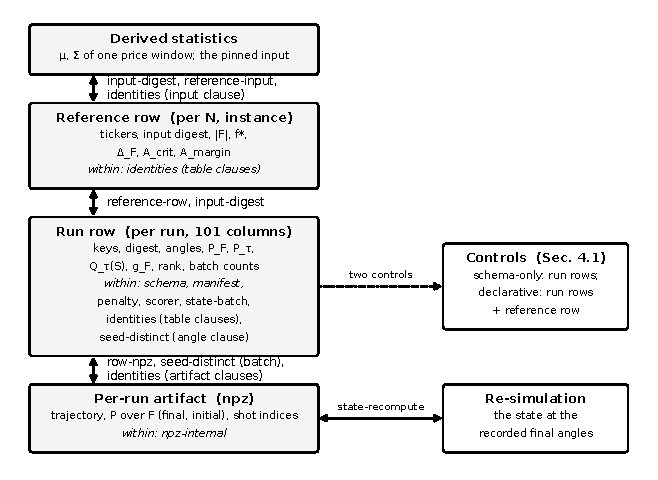
\includegraphics[width=\textwidth]{figures/fig_record_relations.pdf}
\caption{The four files that describe a run and the thirteen checks that bind them. A solid double-headed arrow is a relation between two files, named on the arrow; the relations that hold within one file are listed inside its box. A check with clauses that read different files appears once per clause (identities, seed-distinct); state-batch reads only the run row. The one dotted arrow is not a relation but the two controls of Section 4.1, which read the run rows and the reference row.}
\label{fig:1}
\end{figure}


\textbf{The relations.} Figure 1 places them. Thirteen, each implemented as a function that returns the rows on which it does not hold. Most are consistency conditions that a correct record satisfies outright; three clauses are diagnostics that a correct record can in principle trip, and they are marked as such below, so the set is thirteen checks rather than thirteen invariants. Section 4.1 lists them as the checks of E-S1 and gives the stage at which each runs. Each is marked with what a violation means: \textbf{[E]} exact --- the two sides are equal or the record is inconsistent; \textbf{[N]} numerical --- one side is recomputed and compared within the tolerance given; \textbf{[S]} statistical --- a rule a correct record can fail, so a finding is a suspicion and not a proof. Several relations hold clauses of more than one kind and carry more than one mark; where they do, the clauses are named.


\begin{enumerate}
\item \textit{schema} \textbf{[E]} --- every required column is present and filled on every completed run.
\item \textit{manifest} \textbf{[E]} --- each (N, instance) block holds exactly the (penalty, seed) cells its reference row prescribes, and the file carries one window and one specification version.
\item \textit{penalty} \textbf{[N]} --- the penalty value is the one its label names (relative 10$^{-12}$), and the recorded A/$A_{\mathrm{crit}}$ is their quotient (10$^{-9}$).
\item \textit{reference-row} \textbf{[E]} --- the instance quantities copied onto a run row equal the reference row's, bit for bit: both are the same float64 written twice.
\item \textit{input-digest} \textbf{[E]} --- the digest on the reference row and on every run row is the digest of the pinned statistics.
\item \textit{reference-input} \textbf{[E]} --- the reference row is what those statistics give when the feasible set
\end{enumerate}
is enumerated again. It is worth separating from 4: \textit{reference-row} compares two stored copies of the same value, while this one compares a stored value with a freshly computed one. The harness computes it bit for bit with no tolerance. On the two hosts the numerical study compared, the objective values of the enumeration were bit-identical and only quantities computed through the BLAS (the Sharpe ratio) and through libm ($Q_{\tau}$) differed by a few units in the last place \cite{ref1}, which is why those are numerical relations under 10 and this one is exact; a reader whose host does not reproduce the enumeration bit for bit should expect this relation to report, as Section 5.3's state columns do for a change of precision.

\begin{enumerate}
\item \textit{scorer} \textbf{[N]} --- the solver's best shot, its energy and the scorer's decomposition agree (relative 10$^{-6}$ between the solver's energy and the scorer's, 10$^{-9}$ within the scorer), and $g_{F}$ and $g_{\mathrm{off}}$ follow from f, f*, $\Delta_{F}$ and A (10$^{-9}$).
\item \textit{row-npz} \textbf{[E/N]} --- the row and its artifact describe the same run: the angle vectors and the shot totals bit for bit, $P_{F}$ and $P_{\mathrm{opt}}$ as sums of the stored probabilities at a relative 10$^{-12}$.
\item \textit{npz-internal} \textbf{[E/N/S]} --- the artifact is self-consistent: the trajectory starts at the initial angles (bit for bit), the convergence curve ends at the final expectation (10$^{-12}$), the stored probabilities are a sub-distribution, and the Hamiltonian scale on the row is the one in the artifact. One further clause is a diagnostic rather than an identity: the final angles must differ from the trajectory's first point, which a run stopped at a stationary point could legitimately violate but which no run of this record does, and which is what an optimizer handed a non-differentiable array produces (Section 6, defect 1).
\item \textit{identities} \textbf{[N]} --- every column that is a function of other recorded values equals that function, at a relative 10$^{-9}$ with an absolute floor of 10$^{-15}$, which is the ulp scale the numerical study reports between libm builds: $Q_{\tau}$(S) of $P_{\tau}$; $P_{\tau}$ and $P_{\mathrm{opt}}$ of the stored probabilities and f; the rank of the best feasible shot; the shot-level success counts of the stored batch; D and the offset magnitude $|$$E_{A}$(x*)$|$; the best expectation of the stored convergence; the portfolio metrics of the pinned statistics; and, on the reference row, the penalty scales of its own cardinality minima and the uniform baselines of its counts.
\item \textit{state-batch} \textbf{[S]} --- two shot-count summaries agree with the probabilities the \textit{final} state recorded for them: the smaller one-sided exact binomial tail of the feasible and of the optimum count under S $\times$ $P_{F}$ and S $\times$ $P_{\mathrm{opt}}$ is at least 10$^{-9}$. It is not a test that the batch is a draw from the final state: a fault that moves probability between infeasible solutions, or between feasible ones that are not the optimum, leaves both counts where they were and passes. That is one threshold per \textit{count}, so a count is rejected with probability up to 2 $\times$ 10$^{-9}$ and a row, which carries two, with probability up to 4 $\times$ 10$^{-9}$. And within each (N, penalty) block of at least ten runs whose final $P_{F}$ actually varies, the feasible fraction correlates with final $P_{F}$ above 0.9 and at least as well as with initial $P_{F}$.
\item \textit{seed-distinct} \textbf{[E/S]} --- two runs of one cell that differ only in seed have different initial angles and different shot batches. Neither clause follows from the mathematics of a continuous distribution: a pseudo-random generator is a finite map, and nothing in it forbids two seeds from agreeing. The angle clause is exact \textit{in the scope of this record} and no wider --- the generator is \texttt{numpy.\allowbreak{}random.\allowbreak{}default\_\allowbreak{}rng} (PCG64), the draw is \texttt{uniform(0, $\pi$, 2p)}, and for the five seeds 42--46 at p = 1\ldots{}4 the vectors are pairwise distinct, which a test asserts. Outside that scope it is a diagnostic. The batch clause is a diagnostic everywhere: two batches are discrete objects and can coincide without a defect when the state is concentrated on few outcomes. It is the batch clause that fires on \texttt{shot\_seed\_noop}, in three instances; the angle clause has never fired, which is what the \texttt{shot\_seed} defect predicts, since that defect left the angles alone.
\item \textit{state-recompute} \textbf{[N]} --- the state re-simulated at the recorded final angles reproduces the stored probabilities to 10$^{-5}$ absolute; E1 ran in single precision on a GPU and the check in double precision on a CPU, which agree to about 10$^{-6}$, while a substituted state is off by O(1).
\end{enumerate}

\textbf{What the three kinds mean for a reader of a finding.} A violation of an exact relation is a defect in the record: nothing but a wrong write produces it. A violation of a numerical relation is a defect unless the record was produced under conditions the tolerance does not cover, which is why each tolerance above is stated with the arithmetic it allows for. A violation of a statistical rule is a \textit{suspicion}: a correct record can produce one, and the threshold says how unlikely that is. For the binomial tails the bound is a union bound over the counts actually tested, at 2 $\times$ 10$^{-9}$ each: this record carries two counts on each of 2,565 rows, so 5,130 tests bound the chance that any fires on a correct record at 1.03 $\times$ 10$^{-5}$. The true rate is smaller, because the tails of a discrete distribution do not reach their threshold, but the bound is what the design guarantees. It covers those counts and nothing else. The three diagnostics carry no such bound and are not meant to. The correlation floor of 0.9 was read off the clean record's nineteen blocks --- three sizes with six penalty labels each, and an \textit{A0} block that only N = 12 has, because that is the size where $A_{\mathrm{crit}}$ is zero for some instances --- whose correlations run from 0.983 to 0.999. It is a property of blocks of this size and spread rather than a constant. Two guards are part of the rule: a block of fewer than ten runs is not tested, and neither is one in which final $P_{F}$ does not vary at all. A third condition is not enforced and should be, since a block whose runs all have nearly the same $P_{F}$ carries little information about the correlation, and a correct record of that shape would fail the rule. A per-block clause without a stated error rate belongs behind a warning rather than a refusal, and the aggregation now reports it as one (below; it refused on it until \texttt{v1.3}, Table 14, gap 9) --- the paper's own example of a design the evaluation did not catch because the evaluation never built such a block. Two seeds carrying the same shot batch is possible without a defect whenever the state is concentrated. And a run whose final angles equal its trajectory's first point is what an optimizer handed a non-differentiable array produces, but also what a run stopped at a stationary point would look like. Each reports something to inspect. Section 5.1 reports the one false alarm the binomial test produced before its threshold was corrected, and the five clean records on which no check fires at all.


\textbf{Where the batch-against-state rule applies.} \textit{state-batch} compares a batch with the distribution the same run recorded, which requires that distribution to be exact --- it is, because the state comes from a state-vector simulator that computes it. On hardware the recorded ideal state is not the distribution the device sampled, and a failure would mean noise as readily as a mix-up; the relation holds for the simulator arms this paper checks and is not claimed for hardware, where it would have to be restated against a noise model or dropped.


\textbf{What P1 prevents, automatically and otherwise.} Before it reads a number, the aggregation runs seven validation routines over the two CSVs --- six in \texttt{v1.2}; one of the seven, the input relation, runs only when the pinned statistics for the record's window are on disk --- and a record that fails one does not reach a table: \texttt{analyze\_e1} names the routine and exits non-zero unless told \texttt{-\allowbreak{}-\allowbreak{}allow-\allowbreak{}inconsistent}. Against the numbering above, what runs is


\begin{itemize}
\item five checks entire: 1 \textit{schema}, 3 \textit{penalty}, 4 \textit{reference-row}, 7 \textit{scorer}, and 5 \textit{input-digest} when the statistics are present --- the relation that catches a record built from an input the published statistics no longer hold (Section 5.1), which the first release of the gate did not run;
\item the binomial clause of 11 \textit{state-batch}, whose false-alarm rate is stated above; and
\item a seventh routine for the range and ordering clauses that 7 and 10 carry and that Section 4.1's control states as families --- probabilities between 0 and 1, optimum $\leq$ within-$\tau$ $\leq$ feasible $\leq$ shots, $P_{\mathrm{opt}}$ $\leq$ $P_{\tau}$ $\leq$ $P_{F}$, f* $\leq$ f of the best feasible shot.
\end{itemize}

It is seven routines over selected clauses, then, not seven of the thirteen. The block-level correlation clause of 11 --- the diagnostic that a block's feasible fractions should track the final state's $P_{F}$ rather than the initial state's --- has no stated false-alarm rate, so the aggregation reports it and does not refuse on it. What does not run: 2 \textit{manifest}, which needs no other file but which a reproduction of one block fails by design; 6 and 13, which re-enumerate from the pinned statistics or re-simulate; 8 and 9, which read the artifact; and the clauses of 10 and 12 that do --- the parts of \textit{identities} that recompute from stored convergence, and the batch half of \textit{seed-distinct}. Those are the separate command of the supplementary material (Section S3), and the README gives the order. One implementation serves both (\texttt{src/\allowbreak{}record\_\allowbreak{}checks.\allowbreak{}py}), so the gate and the checker cannot drift. Section 6 lists the seven defects of the numerical study, how each was found at the time, and which check holds its class now --- for three of them, one of which is held by a diagnostic clause rather than a refusal; four are held by none, and the table says so.


\textbf{What P1 does not prevent.} A fault that preserves every relation is invisible: a consistent substitution of the input statistics \textit{and} the reference \textit{and} every run computed from them is a different, internally consistent experiment. The relations bind the record to itself and to the pinned inputs; they cannot say whether those inputs are the ones the experiment meant to use. Nor, for the committed record, can they say that the run read them at the time: the \texttt{input\_digest} column was appended to that record after the fact, computed from the statistics the package publishes (Availability), so it certifies that the published record and the published statistics correspond and not that a run in 2026-09 consulted the file now beside it. A record written with the column from the first run carries both; this one carries the first. The gap that led to it is gap 1 of Table 14.


\subsection{P2 --- Structural refusal of billing, before submission}

Three mechanisms, each measured in E-S2.


\textbf{Hardware is unrepresentable as the optimizer's backend.} \texttt{Braket\allowbreak{}Solver(backend="braket\_\allowbreak{}ionq")} raises \texttt{ValueError} in the constructor, before an AWS session, a device or a bucket reference is created; the drivers refuse the same setting before constructing a solver. A QPU is accepted only as \texttt{sample\_backend}, the device of the single final sampling call, and a test spies on device construction to assert that the metered device is built exactly once per run. The reason is the framework's: a QPU device offers no adjoint differentiation, so PennyLane's \texttt{best} method resolves to parameter shift and one objective-and-gradient evaluation of the p-layer ansatz on a dense N-asset cost Hamiltonian executes 1 + 2p$\cdot$[C(N,2) + 2N] circuits --- 177 at N = 8, 921 at N = 20 for p = 2 --- each a billable task.


\textbf{Sampling angles are frozen.} The final sampling call receives \texttt{frozen\_\allowbreak{}angles(params)}, a plain array with the trainability flag removed. A QNode --- PennyLane's executable circuit --- that returns one sample per wire cannot be differentiated by the adjoint method; with trainable inputs the metered device's execution path evaluated a parameter-shift gradient that nothing read. This was measured, not predicted: the N = 8 SV1 pilot of 2026-08-09 shows 227 tasks in the service's log --- 50 analytic tasks for fifty optimizer steps and 177 for one sampling call --- and 51 once the angles were frozen (the per-task records are archived and reduced to a per-run ledger, \texttt{paper01\_\allowbreak{}sv1\_\allowbreak{}task\_\allowbreak{}ledger.\allowbreak{}csv}).


\textbf{Cloud runs name themselves.} A cloud or hardware backend requires \texttt{--results-tag}; an untagged run finding the committed baseline files in place is refused unless \texttt{--write-canonical} is passed; \texttt{--resume} appends only missing rows.


\textbf{The acknowledged estimate is part of the record.} A metered invocation prints its expected task count and price floor from its arguments and does not start without an acknowledgement flag; since this revision the acknowledged estimate is also written next to the tagged results, and a check compares it with the task count the provider's own records show for that invocation (\texttt{check\_metered.py}). This is one relation across the billing boundary rather than one of the thirteen inside the record: the pilot of \cite{ref1} that was acknowledged at 51 tasks and billed for 227 fails it, and the corrected run (204 acknowledged, 204 billed) passes. The relation is checked after the fact --- it cannot stop the bill --- but it turns a defect that was found by reading an invoice into one that a script reports. E-S2 does not evaluate this one: it is stated as a design decision and exercised only by the historical pair it reproduces (51 acknowledged against 227 billed, and 204 against 204).


\textbf{Three kinds of control, and which one P2 is.} A metered backend can be guarded at three points (Table~S1 of the supplement lists the provider's four mechanisms by kind): \textit{in the configuration}, before a call is built (a wrong call is unrepresentable); \textit{at the service}, per device, by a dollar cap that rejects a task whose estimate exceeds it; and \textit{at the account}, by a detective control that watches task creation and notifies or revokes. P2 is the first kind. The second is a provider setting where one exists --- for the provider used here, only for hardware, not for the simulator on which this project's one real fallback occurred --- and Section 5.2 treats it as a fourth configuration to show what it adds and what it misses. The third exists as a deployable solution for this provider; it was not part of the platform's footprint, and Section 5.2 deploys it once to measure what it adds. Provider specifics are in Section S1 of the supplementary material.


\textbf{What P2 prevents.} The optimizer loop on hardware (stopped at the command line and at the constructor), the sampling fallback (removed before the call reaches the device), and the overwrite of the baseline by a trial run (refused before a solver exists).


\textbf{What P2 does not prevent.} A correctly built call that is expensive by its parameters: one sampling task on IonQ at the default 1,000 shots costs \$0.30 + 1,000 $\times$ \$0.08 = \$80.30 and passes every structural guard, because nothing in its structure is wrong. Only a cap sees the shot count --- and only while the cap is below the price of the one task: at \$50 the 1,000-shot call is refused because it would cost \$80.30, and a \$100 cap would let it through (Section 5.2). Nor does P2 prevent the \textit{repetition} of correct calls --- a script that invokes the solver in a loop, a scheduler that re-issues a finished run --- the failure a recursive serverless function makes familiar. A structural guard constrains how one call is built, not how many calls are made. The platform bounds one invocation (the acknowledged estimate above, and a cross driver that accepts local backends only) and bounds how long it waits for one task (a one-hour polling limit in place of the client library's five-day default, which frees the process but does not cancel the task or stop its charge), but a bound per invocation is not a bound per account. That bound is the second and third kind of control above; the platform's own footprint had only a post-hoc budget notification, whose lag is hours against a pilot that submitted 227 tasks in fourteen minutes, and Section 5.2 measures the third kind's lag in tasks. Nor does P2 address a provider's own failure modes --- the four IonQ task records were parsed from S3 directly after the client library misread the device's nested result schema into an energy of exactly 0.0 \cite[Sec. VI-C]{ref1}.


\textbf{The general form of the defect P2 guards against.} The sampling fallback is one instance of a class: \textit{the framework decides the billable unit from a property of an object rather than from what the user asked for}. Here the property is a tensor's trainability flag and the unit is a parameter-shift tape; elsewhere in the same kind of stack it is a primitive's default shot count, an error-mitigation setting that multiplies the circuits submitted, or a hybrid job billed by wall-clock while a classical loop waits. What makes the class dangerous is not the default but that the cost is decided below the level at which the experiment is described, so that reading the experiment's description does not tell anyone what it will cost. The structural answer is the same in each case: make the expensive configuration unrepresentable, and write the acknowledged estimate into the record so that the bill can be checked against it. We have measured this for one stack; the other instances are named here as observations, not as results.


\subsection{P3 --- Three reconstruction levels with recorded cost}

The public package documents three commands: (1) regenerate the figures and check every manuscript cell against the committed CSVs; (2) run one small instance end to end on a CPU; (3) run the E1 cross from its manifest on a GPU. The cross-experiment driver writes its CSV and its artifact directory after every run, and its \texttt{--resume} reads the manifest --- the run table, as the driver calls the file it writes --- skips the (N, instance, penalty, seed) cells already present, refuses a manifest written by a different specification version, and appends the rest, so that a restart after any interruption converges to the same file as an uninterrupted run. The single-instance driver has neither: it flushes after every size rather than every run and merges into an existing file rather than resuming, so a long run of it is covered by the detached wrapper's status file and not by one of its own. The reference row of an instance is written once and reused. The README states the environment that produced the numbers (\texttt{requirements-\allowbreak{}repro.\allowbreak{}txt}, a \texttt{pip freeze}), the minimum versions the code runs with, and which columns are expected to differ across hosts (single-precision state quantities and every shot-derived column) and which are not (reference quantities, initial angles).


\textbf{A flush bounds the loss only if it cannot be interrupted.} The per-run flush rewrites the whole manifest, so it bounds the loss at the run in flight only if the rewrite cannot be interrupted half-way, and a run's log line must follow its row rather than precede it (both were otherwise in \texttt{v1.0}; Table 14, gap 4). Every result file, the cross driver's manifest included, is written by one function that lands it with a single rename, and the run's line follows the record rather than preceding it; a test kills that function inside the write and asserts that what was on disk before is still there. The heartbeat is written after the rename, so a status of \texttt{RUNNING k/n} always names k rows that are on disk. Fault injection against the record cannot find this class of fault: the failure is in the \textit{writer}, in a window no injected fault occupies.


What that bound covers is one writer and one kind of interruption: the process is killed, the filesystem keeps what was renamed, and no second writer is appending to the same manifest. It is not a transaction over the manifest, the artifacts and the status file together, and it is not a claim about durability after a power loss; each of those would need a different mechanism and a different test, and neither is evaluated here.


\textbf{The end state of a job is a written fact.} Flushing bounds the loss on interruption to one run; it says nothing about how long the interruption goes unnoticed, nor whether the file a reader aggregates is whole. The cross driver therefore keeps a status record beside its manifest (\texttt{<manifest>.\allowbreak{}status.\allowbreak{}json}: \texttt{RUNNING} with a heartbeat after every run, the rows done of the rows planned and the last run id; \texttt{EXIT 0} or \texttt{FAILED code} at the end; a kill leaves \texttt{RUNNING} with a stale heartbeat, which is the stall; the heartbeat is written after the manifest, so the count it carries is a count of rows on disk), prints the previous invocation's state on \texttt{--resume}, and the aggregation refuses a manifest whose job is not \texttt{EXIT 0} and complete unless told to proceed.


A status record is itself a claim about a file, and a claim nothing compares to its subject is the inference the record was written to remove. So the aggregation reads the manifest before it trusts the record: the row count against the rows the record says were written, a run id that occurs twice, a last run the file does not hold. The need was shown by a deleted row that the status record did not notice (Table 14, gap 8). The comparison is exact where the job ended normally and allows one row where it did not, because the driver writes the row before it beats and a kill between the two leaves the file one ahead. It is not waived by the flag that aggregates an unfinished run: that flag is for a job known to be incomplete, not for a file the record does not describe.


\texttt{EXIT 0} says the driver reached the end of its loop with every planned run attempted and recorded, not that every run succeeded. A run that raises is recorded as a row with an \texttt{error:} status and counted in the record's \texttt{failed}, which the state line prints; \texttt{--resume} fills the gaps the manifest does not hold and does not retry those rows, because a recorded failure is an observation about a configuration and re-running it would replace that observation with a second attempt's. That is the opposite of what a workflow engine does --- Snakemake \cite{ref21} re-runs a failed rule, and Amazon Braket's Hybrid Jobs \cite{ref42} let a new job start from the checkpoints a failed one saved --- and deliberately so: a retry is the right answer when the failure is the environment's, and here it may be the configuration's, which is what the run was there to find out. Any other long job runs under a wrapper that keeps the same four states in a one-line file. Both date from gap 3 of Table 14, and the driver's record is exercised in Section 5.3.


\textbf{A device's availability is a written fact too.} A hardware observation that depends on a device being online is not retried by hand: a poller records the device status at a fixed interval, launches the observation once when the status is \texttt{ONLINE}, and gives up after a stated number of days; its log is the record of how long the device was unavailable (Section 5.2 reports one such wait).


\textbf{What P3 prevents.} Loss of completed work on interruption beyond the run in flight; divergence between a resumed and an uninterrupted run; a reader's dependence on the author's machine for levels 1 and 2; a reader's dependence on the market-data provider at all.


\textbf{What P3 does not prevent.} Reproduction of the metered arms without an AWS account and spend; the N = 20 timing columns without the same GPU class; bit-identity of single-precision state quantities across hosts, which \cite[Supplementary Sec. S-VI]{ref1} showed does not hold. Nor does the platform reconcile its task ledger with the provider's invoice: the dollar figures in this paper were compared with the billing console by hand (once finding a \$4.67 omission in an earlier tally), because the billing API is itself metered and an invoice settles days after the tasks.


\subsection{What is not claimed}

The platform is an experiment platform. It makes no claim about production trading systems, market risk, security beyond least-privilege IAM for a results bucket, or regulatory compliance. Its threat model is the experimenter's own mistakes and the provider's drift, not an adversary.


\section{Evaluation design}

Three evaluations, one per principle, each with a control. The cloud calls are 178 SV1 tasks for the sampling-fallback observation, 1,071 SV1 tasks across the six repetitions of the account-level cost control, and the two spending-limit requests of Section 4.2 (Table~S3 of the supplement); no quantum processor was billed.


\subsection{E-S1 --- Does the record catch a mix-up? (P1)}

\textbf{Subject.} The committed E1 record: 2,565 run rows, 90 reference rows, 2,565 artifacts, the derived statistics of the 2023-08-06 $\rightarrow$ 2026-08-05 window.


\textbf{Checks.} Thirteen functions, one per relation of Section 3.1, run in stage order so that the cheapest that can see a fault sees it first:


\begin{itemize}
\item \textit{file} --- schema, manifest.
\item \textit{row} --- penalty, reference-row, scorer.
\item \textit{input} --- input-digest recomputes the content digest of $\mu$ and $\Sigma$ from the derived statistics and compares it with the one on the reference row and on every run row; reference-input re-enumerates the feasible set from those statistics alone, as a clone would.
\item \textit{artifact} --- row-npz, npz-internal.
\item \textit{row}, again --- identities recomputes every column that is a function of other recorded values.
\item \textit{statistical} --- state-batch has two clauses of different kinds, and the difference matters. The per-count clause is a test: the smaller exact one-sided binomial tail under the recorded probability, flagging below 10$^{-9}$, which is a false-alarm rate conditional on the null model of i.i.d. sampling at that probability and bounds the 5,130 counts of this record at 1.03$\cdot$10$^{-5}$. The per-block clause is not: requiring the feasible fraction of a (N, penalty) block of 45 to 150 runs to correlate with final $P_{F}$ above 0.9, and above its correlation with initial $P_{F}$, is a threshold read off the clean record, with no stated error rate. The same holds of \textit{seed-distinct} and of the identity clauses: the union bound above covers the binomial clause and nothing else.
\item \textit{block} --- seed-distinct.
\item \textit{recompute} --- state-recompute re-simulates, per size, the reference instance's $A_{\mathrm{heur}}$ seed-42 run and four spaced runs per N, at their recorded final angles, on \texttt{lightning.qubit} in double precision, and compares the feasible probabilities with the stored ones at 10$^{-5}$ --- fifteen of the 2,565 runs, a
\end{itemize}
sample whose reach this evaluation therefore does not measure (Section 5.1). E1 ran in single precision on a GPU, so agreement to about 10$^{-6}$ is expected and a swapped state is off by O(1).


\textbf{Faults.} Ten, each applied to an in-memory copy of the record (Table 1). Four reproduce defects that occurred in this project; six are mix-ups a user of the code base can make. The harness's first pass is the clean record, on which every check must return nothing.



\begingroup
\small
\setlength\LTleft{\fill}
\setlength\LTright{\fill}
\begin{xltabular}{\textwidth}{>{\hsize=0.607\hsize}Y>{\hsize=1.885\hsize}Y>{\hsize=0.508\hsize}Y}
\caption{Injected faults. Each changes only the records its row names, leaving the rest of the copy as committed; ``the row'' is the run row and ``the artifact'' its \texttt{.npz}. Section 5.1 says where that partial reach matters.}\label{tab:1} \\
\toprule
\textbf{Fault} & \textbf{What is changed} & \textbf{Origin} \\
\midrule
\endfirsthead
\toprule
\textbf{Fault} & \textbf{What is changed} & \textbf{Origin} \\
\midrule
\endhead
\endfoot
\bottomrule
\endlastfoot
price\_perturbation & one asset's mean return in the derived statistics $\times$ (1 + 10$^{-6}$) & the provider's 4.2$\cdot$10$^{-7}$ revision, 2026-08 \\
window\_mixin & one run of the prior-window replication (E5) pasted over the same cell of the main file, run id included & plausible merge error \\
optimizer\_mixin & one run of the E3 L-BFGS-B arm pasted the same way & plausible merge error \\
label\_swap & the $A_{\mathrm{margin}}$ and $A_{\mathrm{heur}}$ rows of one (instance, seed) relabelled & setting mix-up \\
angle\_swap & initial and final angles exchanged in the row and in the artifact & handoff error \\
batch\_from\_initial & every row's shot summary --- feasible, within-$\tau$ and optimum counts --- redrawn as one multinomial over the \textit{initial} state, keeping the counts nested; the artifact's shot arrays left as recorded & the E3 L-BFGS-B wrapper defect \cite[Sec. VI-C]{ref1} \\
evaluator\_from\_Q & f of the best feasible shot replaced by its penalised energy, $g_{F}$ recomputed & an evaluator fed the QUBO matrix \\
column\_drop & the \texttt{final\_P\_F} column removed & the E4 \texttt{write\_csv} defect \\
shot\_seed\_noop & seed 43's shot batch replaced by seed 42's in three instances, summary columns copied & the \texttt{shot\_seed} defect \cite[Sec. VI-C]{ref1} \\
reference\_stale & the reference f* of one instance $\times$ (1 + 10$^{-9}$) & a stale regeneration \\
\end{xltabular}
\endgroup


\textbf{Controls and measures.} Three configurations. The \textit{naive} pipeline reads the CSV and computes the study's headline numbers with no check but the schema. The \textit{declarative} control is the vocabulary of a data-quality library, applied generously and in eight families. The name in italics is the tag Tables 3 and 4 report the family by.


\begin{itemize}
\item \textit{schema}: presence and completeness of every required column.
\item \textit{dtype}: the declared type of each column.
\item \textit{set}: the admitted values of a categorical column.
\item \textit{unique}: the run id, the (N, instance, penalty, seed) key, and the shot summary within one cell.
\item \textit{single}: the expected number of rows, and the columns that must hold one value across the file (the window, the specification version, the optimizer, the backend, the precision, the shot count).
\item \textit{range}: probabilities between 0 and 1, counts non-negative, a probability sum of 1 $\pm$ 10$^{-4}$.
\item \textit{pair} and \textit{band}: two columns of one row against each other --- feasible shots $\leq$ shots, optimum shots $\leq$ within-$\tau$ shots $\leq$ feasible shots, $P_{\mathrm{opt}}$ $\leq$ $P_{\tau}$ $\leq$ $P_{F}$, rank $\leq$ $|$F$|$, f* $\leq$ f of the best feasible shot --- and, where the row computes the width itself, the feasible-shot fraction within five binomial standard deviations of final $P_{F}$. \textit{conditional} is the same shape with the label deciding which column the value must equal.
\item \textit{fk}: after a join with the reference table --- which such a library can do, though Deequ's single-table vocabulary cannot --- the instance quantities copied onto each run row equal the reference row they came from.
\end{itemize}

\textbf{What the declarative control is, exactly.} It is stated twice. The vocabulary is written out over the run table in pandas, and the same expectations are also built as a \texttt{pandera} schema and validated with the library (\texttt{es1\_\allowbreak{}pandera\_\allowbreak{}control.\allowbreak{}py}), so that what is reported is a run of the library and not a description of one. The vocabulary was taken from Deequ's constraint set \cite{ref16} and from the built-in checks of pandera \cite{ref17} (\texttt{equal\_to}, \texttt{not\_equal\_to}, the four order comparisons, \texttt{in\_range}, \texttt{isin}/\texttt{notin}, \texttt{str\_*}, \texttt{is\_monotonic}, \texttt{unique\_\allowbreak{}values\_\allowbreak{}eq}, with nullability, dtype, uniqueness and strictness declared on the schema); the schema was run on pandera 0.35.0, which needs no change to the pinned pandas or numpy and so sits in \texttt{requirements-\allowbreak{}control.\allowbreak{}txt} rather than in the reproduction's own pinned list. Deequ is not run: it would put a JVM in front of a CSV, and that is an argument about Deequ's dependencies and not about pandera's. The reading is deliberately generous: every constraint either tool can state over these columns is granted, including pandera's whole-frame checks and a join with the reference table, which Deequ's single-table vocabulary does not offer. Two things are \textit{not} granted, and they are the boundary the comparison measures: an expectation on an aggregate, because in this record the aggregates are the results being checked; and a custom Python function that opens another file --- the artifact, the pinned statistics --- because that function is the verification relation itself, and granting it would make the control a re-implementation of the treatment. What the control therefore measures is not what pandera can execute, which is anything, but how far an expectation stated in the declarative vocabulary over the run table reaches into this record. Section 5.1 reports what the two statements of the control detect. They agree everywhere, which shows that the two statements implement the same expectations; whether that set is the right boundary for the comparison is the separate question answered above. The \textit{relations} configuration runs all thirteen. For each fault we record which checks fail, the first failing check and its stage, and how many of thirty headline numbers moved (per N and per penalty setting: the median $g_{\mathrm{off}}$, median $g_{F}$, mean feasible fraction, median final $P_{F}$, and the number of runs with an optimum hit) --- that is, whether a reported metric would have changed had nothing flagged it.


\textbf{Random mutations and column coverage.} The ten faults are ours, which leaves the objection that the checks were written for them. Two further measurements use the same record and the same checks. \textit{Column coverage}: for every column of the run row, the reference row and the artifact (133 in all; the one that is empty on every row is reported as not applicable, and a mutation that lands on it in the random draw below is counted as undetected), one random cell is perturbed --- a value by 10$^{-3}$ relative, a count by $\pm$1, a flag by negation, a string by a different value --- and a column counts as \textit{covered} if some check fails. \textit{Random mutations}: 300 mutations are drawn with a seeded generator from ten operators (a cell perturbed by $\delta$ $\in$ \{10$^{-9}$, 10$^{-6}$, 10$^{-3}$, 10$^{-1}$\}; a cell replaced by another row's; a row's metrics copied onto another row; a row deleted; the penalty labels of a block permuted; a reference cell perturbed; an artifact element perturbed; two artifacts exchanged; one entry of the derived statistics perturbed; a column dropped), each applied to a copy and run through the cheap checks. Both were run three times, because the first pass's uncovered list told us which columns a further identity could bind; the passes are reported in that order. Because the checks were developed against that draw, a fourth run of the mutation harness was made after they were frozen: 300 further mutations from the same operators with a different seed, run once, with nothing changed in the checks afterwards.


\textit{A fault injected by re-running.} The three operators that reach outside the run table edit a record that already exists, so none of them can move a headline number, which is a function of the run table alone. The fault this project actually met --- rows computed from an input the published statistics no longer hold --- is injected the way it happened: one mean return of the pinned statistics is perturbed by a relative $\delta$ $\in$ \{0, 10$^{-9}$, 10$^{-6}$, 10$^{-3}$, 10$^{-1}$\}, every row of two N = 12 instances is re-run from the perturbed file (every penalty setting the specification gives them, five seeds), and those rows and their reference are spliced into the committed record, which is then read beside the \textit{published} statistics. Two instance pairs with no instance in common were used, each perturbing a different asset that both of its instances hold: instances 0 and 1 (sixty runs) and instances 2 and 3 (forty-five runs, because one of the two has $A_{\mathrm{crit}}$ = 0 and the cross runs three penalty settings there rather than six). Two conditions are checked before any number is read, because the first three attempts at this experiment failed them silently: the re-run must hold the backend, precision, steps, depth, shots and optimizer the committed record holds, or the splice is visible to a uniformity check and the experiment measures the backend; and it must cover each instance entirely, or the instance's remaining rows keep the old digest beside the new reference. The measures are the re-run rows whose stored state differs from the committed ones, the headline numbers moved and the largest relative change among them, the relations that fire, and both statements of the declarative control; the $\delta$ = 0 rung is the control for the re-run itself.


\subsection{E-S2 --- Does a misconfigured run stop before it is billed? (P2)}

\textbf{Stand-in device.} \texttt{default.qubit} subclassed to declare that it supports no derivative method. PennyLane's \texttt{best} differentiation method then resolves to parameter shift exactly as it does for the Braket QPU device, and \texttt{qml.Tracker} counts the tapes --- the circuits, each of which a metered device bills as one task --- that the committed solver's own QNode sends. The count is cross-checked on \texttt{braket.\allowbreak{}local.\allowbreak{}qubit}, the Braket plugin's own local simulator, which also lacks adjoint support, and against the parameter-shift transform's tape count, which is what the SV1 ledger recorded for the sampling call (177 at N = 8). Three independent sources --- the ledger (service), the plugin's device (plugin), the stand-in (framework) --- agree.


\textbf{Misconfigurations.} Five (Table 2). Four are structural errors; the fifth is a correct call with an expensive default, included so that the table shows what the structural guards do not see.



\begingroup
\small
\setlength\LTleft{\fill}
\setlength\LTright{\fill}
\begin{xltabular}{\textwidth}{>{\hsize=0.597\hsize}Y>{\hsize=0.848\hsize}Y>{\hsize=1.555\hsize}Y}
\caption{Misconfigurations a user of the code base can write.}\label{tab:2} \\
\toprule
\textbf{Misconfiguration} & \textbf{What is written} & \textbf{Consequence if nothing stops it} \\
\midrule
\endfirsthead
\toprule
\textbf{Misconfiguration} & \textbf{What is written} & \textbf{Consequence if nothing stops it} \\
\midrule
\endhead
\endfoot
\bottomrule
\endlastfoot
QPU as optimizer backend & \texttt{-\allowbreak{}-\allowbreak{}backend braket\_\allowbreak{}ionq} & 1 + 2p$\cdot$[C(N,2) + 2N] tasks per optimizer step for 50 steps, plus the sampling call's own \\*
Trainable angles at sampling, SV1 & the optimizer's tensors handed to the 1,000-shot QNode & 1 + 2p$\cdot$[C(N,2) + 2N] tasks for one sampling call that returns one shot batch (the 2026-08-09 pilot) \\*
Trainable angles at sampling, IonQ & the same, on hardware at 100 shots & the same count at \$8.30 per task \\*
QPU as sampling backend, default shots & \texttt{-\allowbreak{}-\allowbreak{}sample-\allowbreak{}backend braket\_\allowbreak{}ionq} without \texttt{--shots} & one correct task at \$0.30 + 1,000 $\times$ \$0.08 \\*
Untagged cloud run & \texttt{-\allowbreak{}-\allowbreak{}backend braket\_\allowbreak{}sv1} without \texttt{--results-tag} & the committed baseline behind the paper's tables is overwritten \\
\end{xltabular}
\endgroup


\textbf{Configurations.} \textit{none} (every guard of the code base disabled by monkey-patching: the QPU set emptied, the cloud backends declared local, the canonical-file refusal disabled, \texttt{frozen\_angles} made the identity); \textit{cap} (no structural guard; a \$50 per-QPU spending limit, the project's budget figure, modelled as documented --- tasks accepted while the cumulative list-price estimate stays within the cap, the first task that would exceed it rejected; simulators outside its scope); \textit{structural} (the committed guards, with the device factory returning the stand-in for every cloud backend and the AWS session factory raising if called); \textit{both}.


\textbf{Observed on the service.} Two of the harness's inputs were then checked against the service itself (\$0.67 in total, \texttt{es2\_\allowbreak{}observe\_\allowbreak{}cloud.\allowbreak{}py}): a \$1.00 spending limit was created on IonQ Forte-1 and requested for SV1, and the N = 8, p = 2 sampling QNode was sent to SV1 twice, with trainable and with frozen angles, the tasks the service created in each window counted through \texttt{Search\allowbreak{}Quantum\allowbreak{}Tasks}. The 100-shot probe against the IonQ cap was submitted while the device was offline, and a seven-day poll found no window in which to repeat it (Section 5.2). The third kind of control was then exercised: AWS's cost-control solution \cite{ref33} was deployed as documented (one region, a \$0.30 monthly limit, the denial targeted at the project's IAM user; Lambda images built for x86\_64 instead of arm64, which changes nothing in behaviour), and the cheapest SV1 task --- a Bell circuit at 10 shots, billed at the 3 s minimum, \$0.00375 --- was submitted sequentially, each after the previous had completed, as a variational loop would, until the service denied \texttt{CreateQuantumTask} or 400 tasks had been created (\texttt{es2\_\allowbreak{}observe\_\allowbreak{}cost\_\allowbreak{}control.\allowbreak{}py}). After the first denial the loop kept submitting until three further denials had been returned, about two minutes, to see whether the denial held; the tasks the service accepted in that interval are the ``after the first denial'' count and are included in the created total. The measures are the tasks created after the list-price running total crossed the limit, after the alarm fired, and after the first denial.


\textbf{Measures.} The stage at which the run stops --- \texttt{cli}, \texttt{constructor}, \texttt{pre-submit} (the misconfiguration is removed before the call reaches the device), \texttt{service} (the cap rejects a task), \texttt{submitted} (every task executes) --- the tasks that would reach the service, the tasks billed and the list-price bill (Amazon Braket's list prices as billed to this project in August 2026 and unchanged on the pricing page at the time of writing \cite{ref43} --- IonQ: \$0.30 per task + \$0.08 per shot; SV1: \$0.075 per minute with a 3 s minimum per task, and a sampling task ran 0.11 s), whether a usable result exists, and whether the baseline file survived. Prices change; the counts are the measurement, and every dollar figure in this paper is a count times one of those three prices, so a reader re-prices it from the count. The structural cells run the committed code; the \texttt{none} cells run the same code with the guards removed --- the QPU set emptied, the cloud backends declared local, the canonical-file refusal returning nothing and \texttt{frozen\_angles} returning its input --- so a guard that stopped firing would move a cell. One guard of Section 3.2 is not among them and is not a stage in the vocabulary above: the acknowledgement of the estimate is on the \texttt{run\_experiment} command line, and this harness drives the solver below that line. Table 8 therefore reports what a metered invocation does once its estimate has been acknowledged, which is the case the guards have to survive.


\subsection{E-S3 --- What does a reader need, and what does it cost? (P3)}

\textbf{Protocol.} A clean-room harness plays the reader: a script that has only what the package publishes, on a machine with none of the working tree. It clones the published repository over the network at its release tag (\texttt{v1.0}, commit \texttt{c804a63}, 21 MB of files), creates a fresh virtual environment, installs \texttt{requirements-\allowbreak{}repro.\allowbreak{}txt}, runs the package's test suite, then runs the README's three levels as written: level 1 (\texttt{generate\_\allowbreak{}tqe\_\allowbreak{}figures}, then \texttt{check\_tables.py}), level 2 (\texttt{run\_\allowbreak{}experiment.\allowbreak{}py} on N $\in$ \{8, 12\}, CPU), level 3 as a 24-run block of the cross (N = 12, instances 0--1, seeds 42--43, six penalty settings, CPU, double precision). Every step records its command, wall-clock, exit code, outcome and the inputs the reader had to supply. Level-1 figures are compared byte for byte with the committed renders; level-2 rows with the committed file; level-3 rows column by column with the committed GPU rows, separating reference quantities, state quantities, shot-derived columns and angles.


\textbf{Interruption.} The same block is run with \texttt{--resume}, killed with \texttt{SIGKILL} after seven runs have printed, and re-issued. The rows on disk at the kill are the work the per-run flush saved; the resumed file is compared row for row with the uninterrupted block (both CPU double precision on the same host, so identity is the expectation); the control without flush and resume is what a restart would have redone. The same steps are then repeated on \texttt{v1.2}, the archived release, with the interruption on a twelve-run block (one instance, two seeds) killed after five runs, so that the job status record --- which \texttt{v1.0} does not have --- is exercised; \texttt{v1.2} differs from \texttt{v1.0} in the fixes this paper reports and in the numerical study's revision, and \texttt{v1.3}, the release this paper ships, adds to \texttt{v1.2} the result files of its later measurements and the gate change of Section 3.1 (Availability).


\textbf{Controls for missing material.} The level-2 command in a copy of the clone with \texttt{data/derived} removed and the network unreachable (an unreachable proxy), which is a package without the derived statistics in the hands of a reader without the price snapshot; and the E2 aggregation --- the numerical study's comparison of the optimized state with a uniform draw over the feasible set, which reads every run's stored probabilities --- without the per-run artifacts, which are deposited separately (Zenodo, $\approx$100 MB).


\textbf{Other machines.} Level 1 was then run by hand on three further environments --- Windows (Git Bash, Python 3.12), macOS (3.12) and Google Colab (3.13.15, three times) --- from the same tag and the same written instructions, installing \texttt{requirements.txt} (the minimum versions) rather than the pinned \texttt{requirements-\allowbreak{}repro.\allowbreak{}txt}, which is CUDA-Linux only. These runs test whether the instructions carry to a machine that is not the one they were written on. They do not test independence: \textbf{the author ran all of them} (Section 7).


\subsection{Threats to validity}

\textit{Construct.} E-S2's dollar figures are list prices of August 2026 applied to measured circuit counts; nobody paid them, except the \$0.67 of the service observation and the \$4.02 of the six account-level runs, and they will not hold as the price list changes, where the counts will. The counts for the optimizer loop are measured on a stand-in that shares the framework's execution path, not on hardware; the count for the sampling fallback was re-observed on SV1 for this paper (177 and 1 tasks), because the local devices execute that call once whatever the angles' flag (the harness prints this). The \textit{structural} column of Table 8 is, by construction, the guards of Section 3.2 refusing the settings they were written to refuse: taken alone it is a unit test, and it is reported because the comparison across the four configurations --- which stage each reaches, what each costs, and what each does not see --- is what the table is for. \textit{Internal.} The ten faults of E-S1 are our own choice; four are replays of real defects, six are our judgement of plausible mistakes, and a fault designed to preserve every relation would pass. The false-positive side is measured on five committed records, including the one the faults enter (Section 5.1), which is a statement about these records and this code base, not a false-positive rate for the relations in general. The random mutations answer the choice of faults but not the choice of operators, which are also ours, and their detection rate depends on tolerances we set. The spending-limit model is the documented behaviour; its simulator half was observed, its QPU rejection not yet (Section 5.2). \textit{External.} One code base, one provider, one application; the principles are stated generally but are evidenced here. E-S3's reader is a clean-room script on the author's own host with a warm package cache (\texttt{pip} took 150 s; a cold cache downloads several gigabytes of CUDA libraries); it measures the package, not a stranger's understanding of the README. Level 1 was also run by hand on Windows, macOS and Colab (Section 5.3), which extends the evidence across machines but not across people: every run in this paper is the author's own.


\section{Results}

Three evaluations, three results; each subsection reports one against its control.


\subsection{E-S1: fault detection and coverage}

Where a headline number moves, a declared expectation over the run table is nearly the relations' equal: of 600 random mutations, 52 move one, and the relations catch 51 of them against the declarative control's 49 (Table 4). That closeness does not extend to the table as a whole: of the 432 mutations that edit the run or reference table, the relations catch 346 and the control 167, and Table 5 says where the difference comes from --- 128 of it from clauses that read nothing the control does not read, expectations the control did not declare; 12 from recomputing portfolio metrics from the pinned statistics; and 39 from comparing the edited table with the artifact. Of the 168 mutations confined to a file the table does not hold, the control catches none and the relations 135, 53 of them through the digest of the inputs and the rest by reading the artifacts. And the one fault this project actually met --- rows computed from an input the published statistics no longer hold --- moves published numbers from $\delta$ = 10$^{-6}$ up, leaves every expectation over the table satisfied up to a tenth of a mean return (Table 6), and was passed by the aggregation gate as first released; the gate now refuses it (Tables 3--6).


The clean record passes all thirteen checks. Table 3 gives the matrix.



\begingroup
\small
\setlength\LTleft{\fill}
\setlength\LTright{\fill}
\begin{xltabular}{\textwidth}{>{\hsize=0.900\hsize}Y>{\hsize=0.747\hsize}Y>{\hsize=1.353\hsize}Yllr}
\caption{Detection matrix (N $\in$ \{12, 16, 20\}; 2,565 runs). ``First'' is the first failing check in stage order; ``moved'', how many of the thirty headline numbers changed (three sizes $\times$ two penalty settings, $A_{\mathrm{heur}}$ and $A_{\mathrm{margin}}$, $\times$ five metrics; Section 4.1). Naive and Declarative are the controls of Section 4.1, and the declarative entry names the families of that section that fire; stated as a pandera schema, the same vocabulary returns the same verdict and families on every row. For batch\_from\_initial the first failing check is the injection's (the row no longer matches its artifact); the defect it replays kept the two in agreement, and the check that sees it as it occurred is state-batch (Section 5.1).}\label{tab:3} \\
\toprule
\textbf{Fault} & \textbf{First failing check (stage)} & \textbf{Also failing} & \textbf{Naive} & \textbf{Declarative} & \textbf{Moved} \\
\midrule
\endfirsthead
\toprule
\textbf{Fault} & \textbf{First failing check (stage)} & \textbf{Also failing} & \textbf{Naive} & \textbf{Declarative} & \textbf{Moved} \\
\midrule
\endhead
\endfoot
\bottomrule
\endlastfoot
clean & --- & --- & --- & --- & 0 \\*
price\_perturbation & input-digest (input) & reference-input, identities & no & no & 0 \\*
window\_mixin & manifest (file) & reference-row, input-digest, identities, state-recompute & no & single;fk & 2 \\*
optimizer\_mixin & manifest (file) & --- & no & single & 3 \\*
label\_swap & penalty (row) & --- & no & conditional & 4 \\*
angle\_swap & npz-internal (artifact) & state-recompute & no & no & 0 \\*
batch\_from\_initial & row-npz (artifact) & identities, state-batch & no & band & 12 \\*
evaluator\_from\_Q & scorer (row) & row-npz, identities & no & range;pair & 6 \\*
column\_drop & schema (file) & row-npz, state-batch & \textbf{yes} & schema & 6 \\*
shot\_seed\_noop & state-batch (statistical) & seed-distinct & no & unique;band & 2 \\*
reference\_stale & reference-row (row) & reference-input & no & fk & 0 \\
\end{xltabular}
\endgroup


Three observations.


\textit{Detection is at the cheapest stage that can see the fault.} Six faults stop at the file or row stage, before any artifact is opened; one (price\_perturbation) stops at the input stage, where the content digest is recomputed from the derived statistics in 1.2 s for all 90 instances and 2,565 rows; the two that require the artifacts (angle\_swap, batch\_from\_initial) stop at the artifact stage; one (shot\_seed\_noop) reaches the statistical stage, where it fails both the batch's binomial test and the diagnostic that two seeds should carry two batches. The harness records what each check costs on each record (\texttt{paper02\_\allowbreak{}es1\_\allowbreak{}finding\_\allowbreak{}counts.\allowbreak{}csv}), and the spread is three orders of magnitude: on the clean record the schema takes 0.009 s, the whole set 46.6 s, and most of that is the three checks that derive rather than compare --- reference-input re-enumerates every feasible set from the pinned statistics (10.5 s), identities recomputes every derived column (10.3 s), and state-recompute re-simulates the sampled states (13.1 s). The two that re-derive from outside the record --- reference-input and state-recompute --- are redundant for every fault: each confirmed a fault a cheaper check had already flagged.


\textit{Seven of ten faults move headline numbers silently.} The largest is the replay of the E3 L-BFGS-B defect: drawing every batch from the initial state moves twelve of thirty headline numbers (the feasible-fraction mean and the optimum-hit count of every size and penalty setting), and the naive pipeline reports them as the study's results. label\_swap moves four --- the $A_{\mathrm{heur}}$-versus-$A_{\mathrm{margin}}$ contrast that is the numerical study's main finding --- and passes every check a schema-only pipeline has. Only column\_drop is visible to the naive pipeline, because a missing column is the one fault that a CSV reader cannot ignore.


\textit{Two changes the evaluation made to the harness.} The first pass of this harness carried only an instance digest, a hash of the ticker set, and a 10$^{-6}$ relative change to one mean return in the derived statistics passed every relation that reads the record; it was caught only by re-enumerating the reference from the statistics (f* of instance 7 at N = 12 moves from $-$0.24331838 to $-$0.24331874). The digest bound the record to \textit{which} inputs, not to their values, which is less than P1 as stated in Section 3.1 requires. A content digest of $\mu$ and $\Sigma$ (\texttt{input\_digest}) was added to every run row and reference row --- appended to the committed files from the pinned statistics, without re-running anything --- together with the input-digest relation, and the same fault now fails on 1,009 records at the input stage in 1.2 s, with reference-input confirming it in 9.7 s (10.5 s on the clean record above: separate runs of one check; Table 14, gap 1). The second change removed a false positive: a first version of state-batch used a five-sigma band around S $\times$ $P_{\mathrm{opt}}$ with a floor of one shot and flagged one clean N = 20 run whose batch held two optimum shots against an expectation of 0.1 --- a 0.5\% event, and with 2,565 runs an expected occurrence. The exact binomial tail with a threshold of 10$^{-9}$ over the record's 5,130 counts replaced it; it still reports 2,299 findings under batch\_from\_initial and three under shot\_seed\_noop.


\textit{Where an expectation stated over the table stops.} The declarative control of Section 4.1 --- the vocabulary of a data-quality library over the run table, applied generously --- catches eight of the ten faults where the schema-only pipeline catches one: both pasted rows, because each makes a column take two values where the file must hold one (\texttt{data\_start} and \texttt{data\_end}; \texttt{optimizer} and \texttt{steps}); the stale reference, after a join with the reference table; the dropped column; the evaluator fed the QUBO matrix, where f of the best feasible shot falls below the instance's optimum on 2,463 rows and $g_{F}$ turns negative; the relabelled penalty, as a conditional equality between a label and a column of the same row; the re-used shot batch, as two runs of one cell carrying one shot summary; and the batch drawn from the initial state, by a band of five binomial standard deviations around final $P_{F}$ that holds on every clean row and fails on 2,319 faulted ones. The two it misses are missed for where the value lives, not for the vocabulary: the revised statistic is caught by recomputing a content digest of the pinned file, and the exchanged angles inside the artifact, where the stored trajectory no longer begins at the recorded initial angles (\texttt{npz-internal}, confirmed by \texttt{state-recompute}) --- neither value is in the table, so no predicate over its columns reaches either, however expressive. That increment is narrow: everything else the control reaches is a relation we would now declare rather than write by hand, and, as Section 4.1 sets the comparison up, the eight-against-ten says where a \textit{declared} expectation over the run table reaches in this record, not that a library could not run these two checks as custom code.


\textit{The control, run as the library.} That eight-of-ten is the vocabulary written out in pandas, and a reader may reasonably ask whether a boundary we drew ourselves is a fair stand-in for the library they would reach for. Built as a \texttt{pandera} schema and validated with pandera 0.35.0, the same expectations return the same verdict on all eleven rows of Table 3 --- the same eight faults, the same two missed, and the same families firing on each --- and no finding on the committed record. On the mutations the agreement holds per operator and in both draws: 81 of 300 here and 86 of 300 in the held-out draw, the counts the written-out control reaches, and none of the 168 mutations that touch a file the table does not hold. The two faults both statements of the control miss, a perturbed input statistic and an exchanged pair of angles, are missed for the reason the boundary names: reaching them means opening the pinned statistics or the stored artifact, and that is a relation rather than an expectation. \texttt{check\_tables.py} binds this agreement, so a later change to either statement that broke it would fail the manuscript's own checker.


\textit{What Table 3 says for batch\_from\_initial, and why.} The replay draws the three nested counts --- optimum $\subseteq$ within $\tau$ $\subseteq$ feasible --- from one multinomial over the initial state, because the defect drew one batch from one wrong state and its counts were therefore mutually consistent; drawn independently they break that ordering, and a pipeline then catches the injection on an inconsistency the defect never produced. The replay rewrites the row's shot summary and leaves the artifact's shot arrays as recorded, and this is a limit of the record rather than a choice: the \texttt{.npz} stores the probabilities of the feasible set, not the full state, so a batch over all 2$^{N}$ outcomes cannot be redrawn from the initial state out of the record alone. \texttt{row-npz} and \texttt{identities} therefore fail on a mismatch between row and artifact that the defect itself never had, and \texttt{row-npz} is the first failing check for a reason the defect never gave anyone. The check that sees the defect as it occurred is \texttt{state-batch}, which compares the batch with the state the same run recorded: 2,299 findings on 2,252 of the 2,565 rows and on all nineteen (N, penalty) blocks, whose feasible fraction tracks the initial state rather than the final one --- the check that caught the defect in the numerical study (Table 13, defect 7), and the one that stays when the artifact is made to agree. For this row of Table 3 the \textit{Also failing} column, not the first one, carries the claim.


\textit{What kind of rule catches each fault.} In the sense of Section 3.1, six faults are caught by an exact relation, a plain inconsistency between two recorded things with no tolerance involved --- both pasted rows against the manifest, the stale reference against the run rows, the revised statistic against the digest of the pinned file, the exchanged angles against the artifact's own trajectory, the missing column against the schema; two by a numerical relation, where every record agrees and the value is nevertheless wrong, so only a recomputation finds it --- the relabelled penalty and the evaluator fed the QUBO matrix; and two by a statistical rule --- the copied shot batch, by the binomial tail and by the diagnostic that two seeds should carry two batches, and the batch drawn from the initial state, for which no pair of records disagrees at all once the replay is faithful. That is the ordering of difficulty, and it is why the record stores the state and not only the summary. It also fixes what those last two findings are: a suspicion a reader then confirms, which is how the \texttt{shot\_seed} defect was actually settled, by comparing two sweeps that should have differed and did not.


\textit{Two more records, injected into.} Everything above --- the ten faults, the pandera comparison, the 600 mutations and the tier count --- is a measurement on one record. The same harness was then run, changed only in which record it loads, on two sibling records the same driver produced: the prior-window replication E5 (300 runs; a different market window, so different pinned statistics, references and digests) and the L-BFGS-B arm of E3 (300 runs; a different optimizer). The two arms have the same shape, so the seeded draw gives them the same 600 mutations, and what differs is the record they land on. On both, the ten faults are detected ten of ten, each by the same first relation as on the main record; the declarative control catches the same eight and misses the same two; and the pandera schema agrees with the hand-written control on every row of the matrix and on every mutation. Of E5's 600 mutations 486 are detected (82\% and 80\% in the two draws), of the L-BFGS-B arm's 490 (83\% and 80\%). Of the 93 E5 mutations that move a headline number the relations catch 92 and the control 90; of the arm's 95, 94 and 93. Of the 170 that reach outside the table, in each record, the relations catch 131 and 133 and the control none; the tiers of Table 5 detect 8, 9, 10 and 10 of the faults on both; inside the run table 291, 302, 355 and 355 of 430 on E5 and 292, 303, 357 and 357 of 430 on the arm; outside it 0, 55, 131 and 131 on E5 and 0, 54, 133 and 133 on the arm. The one headline-moving miss on each is the same 10$^{-9}$ perturbation of a feasible-shot fraction as on the main record. Three perturbed input statistics per record are not detected, and should not be: each is a covariance entry of two assets that no instance of these records holds together --- ten instances per size cover 1,170 of the 1,225 asset pairs where the main record's thirty cover all --- and the digest binds the inputs a run read, not the file. The mutation files carry the suffixes \texttt{\_e5} and \texttt{\_e3\_lbfgs}.


\textit{Five clean records, not one.} Zero false positives above is a statement about the records the faults were injected into. The same thirteen checks were then run, with nothing injected, on every record the same driver produced and committed: the prior-window replication (300 runs whose market window, pinned statistics, references and digests all differ), the two E3 optimizer arms (300 runs each, ADAM 0.03 $\times$ 100 and L-BFGS-B), and the pilot block (36 runs, one seed). Over 3,501 runs, 186 reference rows and 3,501 artifacts, across two market windows and three optimizer settings, \textbf{no relation reports a finding}. What that does and does not establish: the tolerances and the statistical threshold were set on the first of these records, and at a binomial threshold of 10$^{-9}$ over a few thousand counts per record a rate of zero is what the threshold was chosen to produce. The other four records add that relations calibrated on one record do not fire on four they were not calibrated on, one of them from a different market window with its own statistics, references and digests; the two of them that the faults were also injected into show, above, the same detections. Two things had to change for that measurement to mean anything, and both were in the checker rather than in the records: the manifest relation compared every block against E1's own six-setting penalty grid, where an arm may run two of the six, and now reads the grid the arm's own manifest records; and one identity read a column the pilot, written before that column existed, does not carry, where absence is the schema relation's business. Neither changes a cell of Table 3.


\textbf{Column coverage and random mutations.} The relations bind 114 of the record's 132 value-carrying columns (of 133 columns, one is empty on every row). Before the evaluation they bound 47; the identity check of Section 3.1, written in two rounds in response to the first coverage pass, binds 63 that no other relation does, and four more (\texttt{p\_layers}, \texttt{steps}, \texttt{stepsize}, \texttt{status}) joined the manifest relation's list of columns that must hold one value across the file. Table~S2 of the supplement gives the three passes. The 18 columns that remain uncovered are of three kinds: seven only a re-simulation can bind (the full-state expectations at the initial and final angles and the interior of the trajectory and of the convergence curve), eight record \textit{how long} or \textit{how many} rather than \textit{what} (timings and evaluation counts), and three could be bound and are not (the best shot including infeasible ones, the objective of every feasible solution, and a best-expectation column that is empty on all but ten rows). Of the 300 random mutations, 236 (79\%) were detected; of the 26 that moved a headline number --- the mutations that would have changed something the paper reports --- \textbf{25 were caught}, and the one that was not moved a feasible-shot fraction by 10$^{-9}$ relative, which moved a mean by 10$^{-12}$ (Table 4). Those 26 are not evenly spread --- 17 are permuted penalty labels, 5 deleted rows and 2 copied metrics --- so the figure is mostly about three operators that move a block of the record at once.


The declarative control detects 81 of the 300, and \textbf{24 of the 26 that move a headline} against the relations' 25. On this mutation set it is barely worse, and Table 4 shows why: what moves a headline here is a block of the table changing at once, which an expectation over the table sees. The two separate elsewhere. Of the 52 perturbed artifacts, the 15 exchanged artifacts and the 24 perturbed inputs --- 91 mutations that touch a file the table does not contain --- the control detects none and the relations detect 71. None of those 91 moved a headline number, and that is not a fact about the draw: the headline numbers are computed from the run table alone, and these three operators change an artifact or a pinned statistic and leave every row as it was, so none of them \textit{can} move one. The gap this leaves is real and Section 5.1 closes it, in Table 6, with a fault that does move a headline --- one where the wrong input produced the rows rather than being edited beside them, which is the shape the two defects of this project that moved reported numbers actually had. Detection depends on magnitude as the tolerances say it should: 100\% for a count moved by one, 79--81\% at 10$^{-6}$ to 10$^{-1}$, 47\% at 10$^{-9}$, which is the relative tolerance itself (Table~S4 of the supplement gives the counts for both draws). Of the 64 missed, 38 touch the unbindable columns above, 19 are 10$^{-9}$ perturbations of bound columns, and seven sit inside a stated tolerance (a probability sum of 1 $\pm$ 10$^{-4}$ replaced by another row's; an interior value of the stored f that is neither an extremum nor the selected solution). Every operator that changes \textit{which} record a value belongs to --- a swapped artifact, a copied row, a deleted row, a permuted label, a perturbed input --- was detected in 100\% of its draws.


\textbf{What these rates are a rate of, and a held-out draw.} The 300 mutations were drawn once and then used three times, and between passes the relations changed: the uncovered list of the first pass is what told us which columns a further identity could bind. The 79\% is therefore the rate of the final relations on the mutation set they were developed against, not an estimate of their rate on faults nobody has seen. So, with the relations frozen and nothing changed in them afterwards, the same harness drew 300 more from the same operators with a different seed and ran them once: \textbf{245 (82\%) detected}, and of the 26 that moved a headline number, \textbf{26 were caught} (Table 4, last row; \texttt{paper02\_\allowbreak{}es1\_\allowbreak{}random\_\allowbreak{}faults\_\allowbreak{}heldout.\allowbreak{}csv}). The control detects 86 and 25 of the 26. The 77 mutations that touch a file the run table does not contain --- a perturbed artifact, an exchanged artifact, a perturbed input --- are caught 64 times by the relations and never by the control, the same separation the ten faults show. What this does not remove is that the mutation operators are ours, so both rates are conditioned on a distribution of faults we chose, and that the tolerances were set on this record.



\begingroup
\small
\setlength\LTleft{\fill}
\setlength\LTright{\fill}
\begin{xltabular}{\textwidth}{Ylllll}
\caption{300 random mutations by operator, final pass. ``Declarative'' is the control of Section 4.1 on the same mutations; ``Moved'' counts the mutations that changed a headline number and ``Missed'' those of them the relations did not catch. The last row is the held-out draw. Run as a pandera schema instead of written out, the control detects the same number for every operator of both draws: 81 here and 86 in the held-out one.}\label{tab:4} \\
\toprule
\textbf{Operator} & \textbf{n} & \textbf{Detected} & \textbf{Declarative} & \textbf{Moved} & \textbf{Missed} \\
\midrule
\endfirsthead
\toprule
\textbf{Operator} & \textbf{n} & \textbf{Detected} & \textbf{Declarative} & \textbf{Moved} & \textbf{Missed} \\
\midrule
\endhead
\endfoot
\bottomrule
\endlastfoot
cell perturbed ($\delta$ $\in$ \{10$^{-9}$, 10$^{-6}$, 10$^{-3}$, 10$^{-1}$\}) & 80 & 52 & 16 & 1 & 1 \\*
cell replaced by another row's & 30 & 20 & 2 & 0 & 0 \\*
row's metrics copied onto another row & 13 & 13 & 13 & 2 & 0 \\*
row deleted & 15 & 15 & 15 & 5 & 0 \\*
penalty labels of a block permuted & 18 & 18 & 18 & 17 & 0 \\*
reference cell perturbed & 26 & 22 & 5 & 0 & 0 \\*
artifact element perturbed & 52 & 32 & 0 & 0 & 0 \\*
two artifacts exchanged & 15 & 15 & 0 & 0 & 0 \\*
derived statistic perturbed & 24 & 24 & 0 & 0 & 0 \\*
column dropped & 27 & 25 & 12 & 1 & 0 \\*
\textbf{all} & \textbf{300} & \textbf{236 (79\%)} & \textbf{81} & \textbf{26} & \textbf{1} \\*
\textbf{all, held-out draw (seed 7, relations frozen)} & \textbf{300} & \textbf{245 (82\%)} & \textbf{86} & \textbf{26} & \textbf{0} \\
\end{xltabular}
\endgroup



\begingroup
\small
\setlength\LTleft{\fill}
\setlength\LTright{\fill}
\begin{xltabular}{\textwidth}{>{\hsize=0.667\hsize}Y>{\hsize=1.333\hsize}Yrrr}
\caption{Detections by the record each clause reads, on the ten injected faults and on the 600 mutations of both draws --- 432 that edit the run or reference table, 168 confined to a pinned statistic or an artifact. The tiers are nested: a fault or mutation counts at every tier from the first whose clauses detect it. A check whose clauses read different files appears once per clause (identities; seed-distinct). The declarative control reads what T1 reads.}\label{tab:5} \\
\toprule
\textbf{Tier} & \textbf{Clauses} & \textbf{Faults (10)} & \textbf{Inside the table (432)} & \textbf{Outside (168)} \\
\midrule
\endfirsthead
\toprule
\textbf{Tier} & \textbf{Clauses} & \textbf{Faults (10)} & \textbf{Inside the table (432)} & \textbf{Outside (168)} \\
\midrule
\endhead
\endfoot
\bottomrule
\endlastfoot
T1 table + reference & schema, manifest, penalty, reference-row, scorer, state-batch, identities (table clauses), seed-distinct (angle clause) & 8 & 295 & 0 \\*
control (same files) & the eight families of Section 4.1 as a pandera schema & 8 & 167 & 0 \\*
T2 + pinned statistics & input-digest, reference-input, identities (portfolio metrics) & 9 & 307 & 53 \\*
T3 + artifacts & row-npz, npz-internal, seed-distinct (batch clause), identities (artifact clauses) & 10 & 346 & 135 \\*
T4 + re-simulation & state-recompute (a sample of 15 runs) & 10 & 346 & 135 \\
\end{xltabular}
\endgroup


\textit{What each kind of record buys.} Thirteen relations detecting ten of ten says how many checks there are, not which records they need. Table 5 re-counts every detection by the record the detecting clause read, in four nested tiers, with the declarative control on the row of the files it reads. Table 5 shows four things. Binding the input by a digest adds one injected fault and 53 of the 168 mutations outside the table; reading the artifacts adds the last fault and 82 more. Inside the table, T1 alone --- the same two files the control reads --- detects 295 where the control detects 167, so most of what the relations add there is not a kind of record but a vocabulary: identities the control's eight families do not state, which a validation library could declare as readily as we wrote them. Against that, T4 adds nothing to T3 anywhere in this evaluation, and this count could not have shown it adding much: the re-simulation samples fifteen of the 2,565 runs (Section 4.1), so a mutated artifact meets it with probability 0.6\%, and its reach is not measured here; and T1's eight of ten faults are the control's eight, so five of the thirteen relations --- schema, manifest, penalty, reference-row and scorer --- are a re-statement in our own code of what a validation library checks.


\textit{A fault a stored record cannot hold.} Everything above edits a record that already exists, and the headline numbers are a function of the run table, so the three operators that reach outside it cannot move one. The fault this project actually met does --- the provider revised a price between runs --- and the re-run injection of Section 4.1 is its replay. Inside the table the spliced record is consistent: every row of each instance carries one input digest, and it is the digest of its own reference row.


Table 6 is the ladder, for both pairs of Section 4.1 (instances 0--1 and 2--3). At $\delta$ = 0 each re-run reproduces every row bit for bit, moves none of the ten headline numbers and fires nothing --- so every difference below is the perturbation. At $1\times 10^{-9}$ the inputs differ, forty-six of the sixty rows of the first pair and thirty-two of the forty-five of the second carry a different state, and the headline numbers moved none of the ten in either: the relations report a record built from the wrong input \textit{before} a reader would see it in a published number. From $1\times 10^{-6}$ the headline numbers move --- three of the ten in the first pair at $1\times 10^{-6}$ and $1\times 10^{-3}$, one and then two in the second --- and at $1\times 10^{-1}$ five of the ten in both. Which relations fire differs between the pairs in a way that says what they read: in both, \texttt{input-digest} and \texttt{reference-input}, the two that re-derive from the pinned statistics, fire at every $\delta$ from $1\times 10^{-9}$; in the first pair \texttt{state-recompute} joins them at $1\times 10^{-1}$ and in the second it never does, which is its sample and not the perturbation: the sample always holds instance 0's $A_{\mathrm{heur}}$ seed-42 run, which the first pair re-ran and the second did not (Section 4.1). Re-simulating every re-run row instead (\texttt{paper02\_\allowbreak{}es1\_\allowbreak{}input\_\allowbreak{}rerun\_\allowbreak{}recompute.\allowbreak{}csv}) finds the perturbation from $1\times 10^{-3}$ in both pairs --- 3 of 60 and 6 of 45 rows off by up to 4.8$\cdot$10$^{-5}$ and 8.6$\cdot$10$^{-5}$ against the relation's 10$^{-5}$ tolerance --- and on 47 of 60 and 35 of 45 rows at $1\times 10^{-1}$, and nothing at $1\times 10^{-9}$ or $1\times 10^{-6}$, where the state moves by less than the tolerance; the relation sees the perturbation as soon as it exceeds what it allows, wherever its sample happens to fall; in the second pair \texttt{identities} joins them from $1\times 10^{-6}$, because the perturbed asset is in the optimum portfolio of instance 2 and the clause that recomputes that portfolio's Sharpe ratio from the pinned statistics no longer holds --- the third relation that reads the pinned file, which Table 5 counts at T2. It is silent in the first pair because the perturbed asset, 6954.T, is in neither instance's optimum portfolio, and fires in the second because 7011.T is in instance 3's. How far the headline numbers moved is the next column, and it is small: the largest relative change is 2.9$\cdot$10$^{-5}$ and 2.5$\cdot$10$^{-5}$ at $1\times 10^{-6}$ and 8.6$\cdot$10$^{-3}$ and 1.1$\cdot$10$^{-2}$ at $1\times 10^{-1}$ (in the first pair, the median final $P_{F}$ at $A_{\mathrm{margin}}$); the one integer among the ten, the count of runs that hit the optimum, goes from 118 to 117 in the first pair. \textbf{No ordering or conclusion of the numerical study reverses at any of these magnitudes, and this experiment does not claim one does.} What it claims is narrower and is the point: a record built from an input the published statistics do not hold reaches a published table, changes what that table says, and leaves every expectation over the table satisfied. \textbf{At every magnitude, including a tenth of a mean return, neither statement of the declarative control reports anything at all.} Where detection by the relations depends on magnitude as Table 4 shows, detection by an expectation over the table does not depend on it, because the magnitude is not what puts the evidence out of reach. Two instance pairs, each perturbing a different asset, are two existence proofs and not a rate; what they establish is that the boundary of Table 4's last three rows has a consequence a reader of the published numbers would have seen, as observed in both instance pairs tested, each with a different revised asset.


\textit{And whether the routine gate stops it.} The two relations that catch this fault re-derive from the pinned statistics, and the aggregation gate as first released (six routines, \texttt{v1.2}) ran neither: on the spliced records of Table 6 it reported nothing, in 2.6 s, while \texttt{input-digest} alone reports every spliced row and reference in 0.4 s on the N = 12 block of 765 rows the ladder uses (1.2 s on the whole 2,565-run record). The division had been drawn by what a clone can execute, since a reproduction carries no pinned statistics it has not fetched; it was not a cost argument, and the first review of this manuscript named it as the gap it was (Table 14, gap 9). The gate now runs \texttt{input-digest} whenever the statistics for the record's window are on disk, which the released package's are: on the same spliced records it refuses every perturbed rung --- 62 findings on the first pair and 47 on the second, every re-run row and both reference rows, in about 2.2 s --- and reports nothing at $\delta$ = 0, with no warning from the correlation diagnostic at any rung. P1's reach is in two parts: these thirteen relations detect the faults of Tables 3 and 6, and seven validation routines over selected clauses of them stand between an edited record and an aggregate without anyone choosing to look --- the input relation among them wherever the inputs it binds to are present.



\begingroup
\small
\setlength\LTleft{\fill}
\setlength\LTright{\fill}
\begin{xltabular}{\textwidth}{lrrrrrY}
\caption{The re-run injection of Section 4.1 at five perturbation sizes, for instances 0--1 (sixty runs) and 2--3 (forty-five). ``State'': re-run rows whose stored state differs from the committed ones. ``Headline'': of the ten numbers at N = 12 (two penalty settings, $A_{\mathrm{heur}}$ and $A_{\mathrm{margin}}$, $\times$ five metrics), those not bit-identical to the committed value, and the largest relative change among them. The declarative control reports nothing at any rung under either statement.}\label{tab:6} \\
\toprule
\textbf{$\delta$} & \textbf{Instances} & \textbf{Rows re-run} & \textbf{State} & \textbf{Headline} & \textbf{Largest relative change} & \textbf{Relations that fire} \\
\midrule
\endfirsthead
\toprule
\textbf{$\delta$} & \textbf{Instances} & \textbf{Rows re-run} & \textbf{State} & \textbf{Headline} & \textbf{Largest relative change} & \textbf{Relations that fire} \\
\midrule
\endhead
\endfoot
\bottomrule
\endlastfoot
0 (control) & 0--1 & 60 & 0 & 0 / 10 & --- & --- \\*
$1\times 10^{-9}$ & 0--1 & 60 & 46 & 0 / 10 & --- & \texttt{input-digest}, \texttt{reference-input} \\*
$1\times 10^{-6}$ & 0--1 & 60 & 60 & 3 / 10 & 2.9$\cdot$10$^{-5}$ & \texttt{input-digest}, \texttt{reference-input} \\*
$1\times 10^{-3}$ & 0--1 & 60 & 60 & 3 / 10 & 5.0$\cdot$10$^{-5}$ & \texttt{input-digest}, \texttt{reference-input} \\*
$1\times 10^{-1}$ & 0--1 & 60 & 60 & 5 / 10 & 8.6$\cdot$10$^{-3}$ & \texttt{input-digest}, \texttt{reference-input}, \texttt{state-recompute} \\*
0 (control) & 2--3 & 45 & 0 & 0 / 10 & --- & --- \\*
$1\times 10^{-9}$ & 2--3 & 45 & 32 & 0 / 10 & --- & \texttt{input-digest}, \texttt{reference-input} \\*
$1\times 10^{-6}$ & 2--3 & 45 & 45 & 1 / 10 & 2.5$\cdot$10$^{-5}$ & \texttt{input-digest}, \texttt{reference-input}, \texttt{identities} \\*
$1\times 10^{-3}$ & 2--3 & 45 & 45 & 2 / 10 & 5.5$\cdot$10$^{-4}$ & \texttt{input-digest}, \texttt{reference-input}, \texttt{identities} \\*
$1\times 10^{-1}$ & 2--3 & 45 & 45 & 5 / 10 & 1.1$\cdot$10$^{-2}$ & \texttt{input-digest}, \texttt{reference-input}, \texttt{identities} \\
\end{xltabular}
\endgroup


\subsection{E-S2: execution guards and cost control}

\textbf{Measured counts.} One optimizer step of the committed solver on the stand-in device executes 177 / 361 / 609 / 921 tapes at N = 8 / 12 / 16 / 20 (Table 7) --- 1 + 2p$\cdot$[C(N,2) + 2N] in every case, 177 also on \texttt{braket.\allowbreak{}local.\allowbreak{}qubit} at N = 8, and 177 is the sampling-call count of the SV1 ledger's first run. The committed sampling path hands the device one tape with the angles frozen. \textbf{One step is measured and the loop is multiplied out}: the task count of the unguarded optimizer loop in Table 8 is that measured per-step count times the driver's fifty steps, plus the sampling call (50 $\times$ 177 + 177 = 9,027 at N = 8; 50 $\times$ 921 + 921 = 46,971 at N = 20). Running fifty steps on the stand-in would measure the same arithmetic at fifty times the cost, and the stand-in is not the service in any case --- what is measured is the framework's decision, not a bill anyone received.



\begingroup
\small
\setlength\LTleft{\fill}
\setlength\LTright{\fill}
\begin{longtable}{rrrrr}
\caption{Tapes per optimizer step on a device without a derivative method.}\label{tab:7} \\
\toprule
\textbf{N} & \textbf{stand-in (\texttt{default.qubit}, no derivatives)} & \textbf{\texttt{braket.\allowbreak{}local.\allowbreak{}qubit}} & \textbf{transform} & \textbf{formula} \\
\midrule
\endfirsthead
\toprule
\textbf{N} & \textbf{stand-in (\texttt{default.qubit}, no derivatives)} & \textbf{\texttt{braket.\allowbreak{}local.\allowbreak{}qubit}} & \textbf{transform} & \textbf{formula} \\
\midrule
\endhead
\endfoot
\bottomrule
\endlastfoot
8 & 177 & 177 & 177 & 177 \\*
12 & 361 & --- & 361 & 361 \\*
16 & 609 & --- & 609 & 609 \\*
20 & 921 & --- & 921 & 921 \\
\end{longtable}
\endgroup


\textbf{Stopping stages.} Table 8 gives N = 8 and N = 20 (Figure S1 of the supplement draws the N = 8 cells), and the CSV holds N = 12 and 16, which lie between. Throughout, the optimizer loop is fifty steps and the sampling call is 1,000 shots on SV1 and 100 on IonQ, and every dollar figure is a list price applied to a task count rather than a bill anyone received. Where a count was obtained by counting the parameter-shift transform's \textit{circuits} rather than tasks --- one sampling call's tapes, or one step's tapes times the driver's fifty steps plus that call --- it rests on one task per circuit: an identity confirmed at N = 8 on SV1 and against the 2026-08-09 ledger, and assumed at N = 20 and on hardware. Nothing stops at the constructor. The command line refuses first in both of those cases, so the constructor's own refusal (Section 3.2) is a second line that none of these five misconfigurations reaches; it is there for a caller that does not come through the driver.




\begingroup
\small
\setlength\LTleft{\fill}
\setlength\LTright{\fill}
\begin{xltabular}{\textwidth}{>{\hsize=1.105\hsize}Yr>{\hsize=1.217\hsize}Y>{\hsize=1.073\hsize}Y>{\hsize=0.926\hsize}Y>{\hsize=0.679\hsize}Y}
\caption{Stage at which each misconfiguration stops, tasks billed and list-price bill, under four guard configurations (cap = \$50 per QPU). Where a cell comes from: unmarked, the harness ran the committed code and counted what it did; $\ddagger$, observed on Amazon Braket; \S{}, counted as circuits and converted at one task per circuit; $\dagger$, the provider's documented behaviour, not observed. A cell ending in ``---'' returns nothing usable, one ending in ``?'' a value but no gradient. The conventions behind \S{} and the dollar figures are stated above.}\label{tab:8} \\
\toprule
\textbf{Misconfiguration} & \textbf{N} & \textbf{none} & \textbf{cap only} & \textbf{structural} & \textbf{both} \\
\midrule
\endfirsthead
\toprule
\textbf{Misconfiguration} & \textbf{N} & \textbf{none} & \textbf{cap only} & \textbf{structural} & \textbf{both} \\
\midrule
\endhead
\endfoot
\bottomrule
\endlastfoot
QPU as optimizer backend & 8 & \S{} submitted; 9,027 tasks; \textbf{\$74,924} & $\dagger$ service; 6 tasks; \$49.80; --- & \textbf{cli}; 0 tasks; \$0 & cli; 0; \$0 \\
 & 20 & \S{} submitted; 46,971 tasks; \textbf{\$389,859} & $\dagger$ service; 6; \$49.80; --- & cli; 0; \$0 & cli; 0; \$0 \\
Trainable angles at sampling, SV1 & 8 & $\ddagger$ submitted; 177 tasks; \$0.66 & $\ddagger$ submitted; 177; \$0.66 (\textbf{cap blind}) & $\ddagger$ \textbf{pre-submit}; 1 task & $\ddagger$ pre-submit; 1 \\
 & 20 & \S{} submitted; 921; \$3.45 & \S{} submitted; 921; \$3.45 & pre-submit; 1 & pre-submit; 1 \\
Trainable angles at sampling, IonQ & 8 & \S{} submitted; 177; \$1,469 & $\dagger$ service; 6; \$49.80; ? & pre-submit; 1; \$8.30 & pre-submit; 1; \$8.30 \\
 & 20 & \S{} submitted; 921; \$7,644 & $\dagger$ service; 6; \$49.80; ? & pre-submit; 1; \$8.30 & pre-submit; 1; \$8.30 \\
QPU as sampling backend, default shots & 8 & submitted; 1 task; \$80.30 & $\dagger$ \textbf{service; 0; \$0} & submitted; 1; \textbf{\$80.30} & $\dagger$ service; 0; \$0 \\
Untagged run over the baseline & 8 & submitted; 2 tasks; \textbf{baseline overwritten} & submitted; 2; overwritten & \textbf{cli}; 0; baseline intact & cli; 0; intact \\
\end{xltabular}
\endgroup


Structural guards and spending limits address different failure modes. The structural guards stop the two runs that would have been ruinous at the command line and before the call reaches a device, and they do so at every N, because they act on the configuration and not on a running total. The counterfactual bill of the unguarded optimizer loop extrapolates to \$74,924 at N = 8 (the numerical study's ``about \$73,000'' excluded the sampling call's own 177 tasks) and \$389,859 at N = 20 --- one measured step's circuit count times the driver's fifty steps, priced at the list rate, with nothing of either sum ever billed to anyone.


The cap stops the same runs after six tasks of \$8.30 with nothing to show --- the first gradient of the first step needs 177 --- which at \$49.80 is a cheap failure but a failure; and the cap is blind to the simulator fallback that actually occurred in this project (177 to 921 tasks, \$0.66 to \$3.45, and 4.7$\times$ the wall-clock of the corrected run: 808 s between the pilot's first and last task against 172 s for the N = 8 run that replaced it, or 4.3$\times$ against that run's two later replicates). Conversely, the one correctly built call with an expensive default --- one IonQ sampling task at 1,000 shots --- passes every structural guard, because there is nothing structurally wrong with it, and only the cap refuses it --- because \$80.30 exceeds \$50, not because the cap can see that a thousand shots was a slip. The untagged run costs two tasks (\$0.007 at list price) and destroys the file the paper reads; no cap sees it.


\textbf{What the service confirmed.} The sampling fallback is no longer an inference from a month-old ledger: on 16 September 2026, under PennyLane 0.45.1 and amazon-braket-pennylane-plugin 1.35.1, the N = 8 sampling QNode sent to SV1 with the optimizer's angles still marked trainable created \textbf{177 tasks in 672 s}, and the same QNode with frozen angles created \textbf{1 task in 4 s}; both returned a full 1,000 $\times$ 8 sample. The N = 8 SV1 cells of that row therefore rest on two observed counts, 177 and 1; their N = 20 counterparts and the IonQ row are the transform's circuit counts, which Table 8 marks as such. The transform's count and the 2026-08-09 ledger agree with it. Of the cap, one half is observed and one half still modelled: the request for a spending limit on SV1 was refused by the service (``Spending limits can not be created for simulator devices''), which is the row ``cap blind'' of Table 8; the rejection of an over-cap QPU task at creation was attempted with a \$1.00 limit on IonQ Forte-1 and a 100-shot (\$8.30) circuit, and the service answered \texttt{Device\allowbreak{}Offline\allowbreak{}Exception} because the device was outside its availability --- the task was not created and nothing was billed, but the refusal observed was the device's, not the cap's. The probe was then left to a poller that queried the device every 30 minutes for seven days (2026-09-17 09:45 to 2026-09-24 09:28 UTC, 336 queries, \texttt{paper02\_\allowbreak{}ionq\_\allowbreak{}availability\_\allowbreak{}probe.\allowbreak{}log}): the device answered \texttt{OFFLINE} every time and the probe never ran. That is itself the point of P3's device-availability record --- a benchmark that needs this QPU is not runnable on demand, and the platform writes that fact rather than inferring it --- but it leaves the \texttt{service} cells of Table 8 as the provider's documented behaviour, not as an observation of ours.


\textbf{The third kind of control, observed twice.} Deployed as documented, the account-level solution metered nothing that its own record shows: its task-logger function failed on import in every invocation CloudWatch recorded for the first run --- 392 of 392, against the 400 tasks that run created; the record does not say where the other eight events went --- because the Braket SDK pulls in a simulator whose numba-compiled functions try to write a cache beside the source and \texttt{/var/task} is read-only in Lambda. The running-cost alarms stayed \texttt{INSUFFICIENT\_\allowbreak{}DATA}, no denial was attached, and 400 tasks (\$1.50 at list price) were created against a \$0.30 limit. The solution's own ``task logger errors'' alarm did fire, four minutes in --- a detective control for the detective control, which nothing in the documented procedure says to watch. With one environment variable added (\texttt{NUMBA\_\allowbreak{}CACHE\_\allowbreak{}DIR=/\allowbreak{}tmp/\allowbreak{}numba}; supplementary material, Section S1.2) the control behaved as designed, and the measurement was repeated five times with the running cost reset between runs (Table 9). In every run the list-price total crossed \$0.30 at task 81 and the alarm fired 91--96 s later (one 60 s evaluation period plus its phase); and the first \texttt{Access\allowbreak{}Denied\allowbreak{}Exception} came 7--146 s after the alarm --- that interval covers the alarm action attaching the deny policy and IAM's eventually consistent propagation of it, neither of which the record separates. The tasks created after the limit was crossed were \textbf{41--92 (median 47)}, after the alarm \textbf{6--56 (median 10)}, and after the first denial a further 1--5 slipped through before the denial held. The residue the documentation calls ``a few'' is therefore, for a sequential loop at 3--4 s per task, about 47 tasks in the median and twice that in one run of five --- \$0.18 to \$0.35 on the simulator, median to maximum. Priced at IonQ's \$8.30 per task the same counts would be \$390 to \$760, median to maximum, which is an illustration of what a residue of that size costs on hardware and not a prediction of what a QPU loop would overrun by: the residue is a count of tasks a 3--4 s submission loop got in before a denial propagated, and on hardware both the submission rate and the queue are different. It is the order of magnitude that matters here, and it is what a cap of the second kind --- had it existed for the device --- would have stopped at \$50. The structural guards do not apply here at all: each of these calls is correctly built, and P2's refusals act on how a call is built, not on how many are made (Section 3.2). Two cells of the first repetition are not in the summary that run wrote, because the aggregation gained those fields afterwards; \texttt{es2\_\allowbreak{}cost\_\allowbreak{}control\_\allowbreak{}aggregate.\allowbreak{}py} recomputes them from the run's own task records and checks the recomputation against every field the four later summaries do hold.



\begingroup
\small
\setlength\LTleft{\fill}
\setlength\LTright{\fill}
\begin{xltabular}{\textwidth}{Yllllll}
\caption{Five repetitions of the account-level control, one column each (limit \$0.30; SV1 Bell circuit, 10 shots, \$0.00375 per task, sequential). Every cell is an observation on Amazon Braket; nothing here is modelled. Two cells of run 1 are recomputed from its task records by \texttt{es2\_\allowbreak{}cost\_\allowbreak{}control\_\allowbreak{}aggregate.\allowbreak{}py}.}\label{tab:9} \\
\toprule
\textbf{Quantity} & \textbf{1} & \textbf{2} & \textbf{3} & \textbf{4} & \textbf{5} & \textbf{median} \\
\midrule
\endfirsthead
\toprule
\textbf{Quantity} & \textbf{1} & \textbf{2} & \textbf{3} & \textbf{4} & \textbf{5} & \textbf{median} \\
\midrule
\endhead
\endfoot
\bottomrule
\endlastfoot
Tasks created & 124 & 127 & 172 & 121 & 127 & 127 \\*
Created past the limit & 44 & 47 & 92 & 41 & 47 & 47 \\*
Limit $\rightarrow$ alarm & 96 s & 95 s & 94 s & 91 s & 94 s & 94 s \\*
Created past the alarm & 6 & 10 & 56 & 6 & 11 & 10 \\*
Alarm $\rightarrow$ first denial & 16 s & 14 s & 146 s & 7 s & 19 s & 16 s \\*
Created past the first denial & 2 & 5 & 1 & 4 & 5 & 4 \\
\end{xltabular}
\endgroup


\subsection{E-S3: reconstruction cost and recovery}


\begingroup
\small
\setlength\LTleft{\fill}
\setlength\LTright{\fill}
\begin{xltabular}{\textwidth}{l>{\hsize=1.215\hsize}Y>{\hsize=0.380\hsize}Y>{\hsize=1.405\hsize}Y}
\caption{The clean-room harness's steps: levels 0--3 and the two controls on the public package \texttt{v1.0}, then the same checks and the interruption on \texttt{v1.2}, the release E-S3 reconstructs. A fresh environment for each, on one host: Ubuntu, one RTX A6000, the GPU host of Table 12. The byte comparison of the figures and the wall-clock of level 3 are that machine's; Table 12 is what three machines without a GPU do with the same level 1.}\label{tab:10} \\
\toprule
\textbf{Level} & \textbf{Command (from the README)} & \textbf{Wall-clock} & \textbf{Outcome} \\
\midrule
\endfirsthead
\toprule
\textbf{Level} & \textbf{Command (from the README)} & \textbf{Wall-clock} & \textbf{Outcome} \\
\midrule
\endhead
\endfoot
\bottomrule
\endlastfoot
0 & \texttt{git clone -\allowbreak{}-\allowbreak{}branch v1.\allowbreak{}0} & 1.5 s & commit c804a63, 21 MB \\
0 & \texttt{python -m venv}; \texttt{pip install -\allowbreak{}r requirements-\allowbreak{}repro.\allowbreak{}txt} & 8 s; 150 s & PennyLane 0.45.1, NumPy 2.4.6, Matplotlib 3.11.1 \\
0 & \texttt{pytest -q} & 77 s & 364 passed, 4 skipped \\
1 & \texttt{python -\allowbreak{}m notebooks.\allowbreak{}generate\_\allowbreak{}tqe\_\allowbreak{}figures} & 22 s & 5/5 regenerated PNG renders byte-identical to the committed ones \\
1 & \texttt{python check\_\allowbreak{}tables.\allowbreak{}py} & 2.6 s & 2,578 manuscript cells agree, 0 disagree, 0 pending \\
2 & \texttt{run\_\allowbreak{}experiment -\allowbreak{}-\allowbreak{}backend lightning\_\allowbreak{}cpu -\allowbreak{}-\allowbreak{}classical-\allowbreak{}n 8 12 -\allowbreak{}-\allowbreak{}quantum-\allowbreak{}n 8 12 -\allowbreak{}-\allowbreak{}results-\allowbreak{}tag es3} & 18 s & classical and QAOA rows: energy and Sharpe identical to the committed (GPU) file, at N where the best shot is the optimum on both \\
3 & \texttt{run\_\allowbreak{}e1\_\allowbreak{}cross -\allowbreak{}-\allowbreak{}backend lightning\_\allowbreak{}cpu -\allowbreak{}-\allowbreak{}precision double -\allowbreak{}-\allowbreak{}n 12 -\allowbreak{}-\allowbreak{}instances 0 1 -\allowbreak{}-\allowbreak{}seeds 42 43 -\allowbreak{}-\allowbreak{}results-\allowbreak{}tag es3block} & 222 s (9.1 s per run inside the driver) & 24 rows; see Table 11. The committed cross records 13.9 h of run time for 2,565 runs on the GPU \\
3 & same with \texttt{--resume}, \texttt{SIGKILL} after 7 runs & 68 s & 6 rows on disk: the run in flight is lost; control without flush: 0 rows, 68 s to redo \\
3 & re-issue with \texttt{--resume} & 168 s & ``6 rows already done''; 24 rows; 94/94 non-timing columns identical to the uninterrupted block \\
control & level 2 without \texttt{data/derived}, network unreachable & 6 s & fails: \texttt{Type\allowbreak{}Error:\allowbreak{} '<' not supported between instances of 'int' and 'None\allowbreak{}Type'} \\
control & E2 aggregation without the artifacts & 1.2 s & fails: ``no run artifacts under \ldots{}/e1\_runs'' \\
0 (v1.2) & \texttt{git clone -\allowbreak{}-\allowbreak{}branch v1.\allowbreak{}2}; \texttt{python -m venv}; \texttt{pip install -\allowbreak{}r requirements-\allowbreak{}repro.\allowbreak{}txt} & 2.3 s; 8 s; 153 s & commit cdf72a9, 28 MB \\
0 (v1.2) & \texttt{pytest -q -rs} & 119 s & 470 passed, 33 skipped: 29 need the per-run artifacts, 3 the price snapshots, 1 a host without \texttt{lightning.gpu} \\
1 (v1.2) & \texttt{python -\allowbreak{}m notebooks.\allowbreak{}generate\_\allowbreak{}tqe\_\allowbreak{}figures}; \texttt{python check\_\allowbreak{}tables.\allowbreak{}py} & 26.7 s; 2.5 s & 4/6 byte-identical; two differ in one text string each (below); 2,641 cells agree, 0 disagree, 0 pending \\
2 (v1.2) & the level-2 command above & 17 s & energy and Sharpe of the selected solution identical to the committed file, to 0; the state behind it is Table 11's \\
3 (v1.2) & \texttt{run\_\allowbreak{}e1\_\allowbreak{}cross -\allowbreak{}-\allowbreak{}backend lightning\_\allowbreak{}cpu -\allowbreak{}-\allowbreak{}precision double -\allowbreak{}-\allowbreak{}n 12 -\allowbreak{}-\allowbreak{}instances 0 1 -\allowbreak{}-\allowbreak{}seeds 42 43 -\allowbreak{}-\allowbreak{}results-\allowbreak{}tag es3block} & 227 s (9.2 s per run inside the driver) & 24 rows; initial angles identical in 24, every state column in 0, max abs. difference 1.4$\cdot$10$^{-4}$ --- the v1.0 block's pattern (Table 11) \\
3 (v1.2) & the interruption block --- one instance, two seeds, twelve runs --- with the job status record: \texttt{SIGKILL} after 5 runs & 52 s & status file \texttt{RUNNING 5/\allowbreak{}12, last N12\_\allowbreak{}i00\_\allowbreak{}5x\allowbreak{}Acrit\_\allowbreak{}s42}, matching the 5 rows on disk, which the manifest parses with no artifact left without a row; \texttt{analyze\_e1} refuses the manifest \\
3 (v1.2) & re-issue with \texttt{--resume} & 70 s & driver prints ``previous job: RUNNING pid \ldots{} 5/12''; status \texttt{EXIT 0 12/12}; \texttt{analyze\_e1} runs \\
\end{xltabular}
\endgroup


The inputs the harness supplied were the repository URL and tag, a name for \texttt{--results-tag}, and the choice of CPU over the README's GPU for level 3; every other token came from the README.



\begingroup
\small
\setlength\LTleft{\fill}
\setlength\LTright{\fill}
\begin{xltabular}{\textwidth}{l>{\hsize=1.472\hsize}Yl>{\hsize=0.528\hsize}Y}
\caption{Level 3: a CPU double-precision block against the committed GPU single-precision rows (24 runs). The values are the \texttt{v1.0} pass's; the \texttt{v1.2} pass of Table 10 reproduces every row of this table exactly.}\label{tab:11} \\
\toprule
\textbf{Group} & \textbf{Column} & \textbf{Identical rows} & \textbf{Max abs. difference} \\
\midrule
\endfirsthead
\toprule
\textbf{Group} & \textbf{Column} & \textbf{Identical rows} & \textbf{Max abs. difference} \\
\midrule
\endhead
\endfoot
\bottomrule
\endlastfoot
reference & f*, $\Delta_{F}$, $A_{\mathrm{crit}}$, $A_{\mathrm{heur}}$, $A_{\mathrm{margin}}$, Hamiltonian scale & 24/24 each & 0 \\*
angles & initial\_angles & 24/24 & 0 \\*
angles & final\_angles & 0/24 & --- \\*
state & final\_expectation & 0/24 & 1.1$\cdot$10$^{-4}$ \\*
state & expectation\_at\_final\_angles & 0/24 & 1.4$\cdot$10$^{-4}$ \\*
state & final\_P\_F & 0/24 & 6.2$\cdot$10$^{-5}$ \\*
state & final\_P\_opt, final\_P\_$\tau$ & 0/24 & 1.1$\cdot$10$^{-6}$ \\*
state & initial\_P\_F & 0/24 & 4.5$\cdot$10$^{-7}$ \\*
state & final\_Q\_$\tau$(1000) & 0/24 & 3.3$\cdot$10$^{-6}$ \\*
shots & feasible\_shots & 0/24 & 31 shots \\*
shots & shots\_optimal & 10/24 & 5 shots \\*
shots & best\_all\_E, $g_{F}$, $g_{\mathrm{off}}$ & 14/24 & 0.19, 0.28, 0.11 \\
\end{xltabular}
\endgroup


The block changes two things at once --- the host and the precision --- so it bounds what a reader should expect rather than separating the two causes; a CPU run at single precision would separate them and is not part of the level the README defines. What reproduces bit for bit across hosts is what P1 binds the record to: the pinned inputs, the reference derived from them, and the seeded initial angles. What does not is what the numerical study said would not: fifty ADAM steps in single precision on one host and double on another end at different angles, the state quantities differ at the 10$^{-4}$ level, and the shot columns are a different draw from a slightly different state. The README states this division in advance; the table measures it.


\textit{Interruption, on \texttt{v1.0}.} Seven runs had printed their completion line when the process was killed; six rows were on disk. That measurement is of the released \texttt{v1.0}, whose flush rewrote the manifest in place, so the six rows survived because the kill fell outside the rewrite rather than because it could not fall inside it. What an interruption costs either way is the run in flight and its artifact: the \texttt{.npz} is written before the row, so a kill between the two leaves an artifact with no row --- the resumed run rewrites it, and the row-npz relation would flag it if it did not. The seventh had completed its computation and not yet its flush, so the run in flight is the unit of loss and the flush granularity bounds it at one. The resumed run read the six rows, skipped their cells, and produced a file identical to the uninterrupted block in all 94 non-timing columns; the timing columns differ, as they must.


\textit{Interruption, on \texttt{v1.2}.} The block interrupted on \texttt{v1.2} is a twelve-run one --- one instance, two seeds --- and not level 3's twenty-four, because what it measures is the status record and the resume rather than the cost of the block. The renaming driver \texttt{v1.2} ships (Section 3.3) is measured in the last block of Table 10: killed after five runs, the manifest parses and holds exactly the five rows the status file claims, and the resumed run completes the twelve.


\textit{The same checks repeated on \texttt{v1.2}.} E-S3's three levels are an evaluation of \texttt{v1.0}, because that is the package a reader of the numerical study has and the one whose gaps this section reports. The fixes those gaps produced are in \texttt{v1.2}, so the last block of Table 10 clones \texttt{v1.2} and repeats what can be repeated: the suite (470 passed, 33 skipped), level 1 (four of six figures byte-identical and 2,641 manuscript cells agreeing), level 2 (identical to the committed file, to zero), and the interruption and resumption --- which \texttt{v1.0} cannot be asked for at all, since the job status record was written in response to this evaluation. That last step is also where the record gate of Section 3.1 is exercised end to end: it calls the aggregation twice, and the aggregation refuses the partial manifest and then, on the resumed twelve rows, runs the six CSV-level validation routines (seven in \texttt{v1.3}, Section 3.1) of Section 3.1 and finds nothing. Both blocks of Table 10 clone over the network from the published repository, so the passes differ in the tag alone. What the 33 skips are: 29 tests of the E-S1 harness need the per-run artifacts, about 100 MB of \texttt{.npz} that the git repository does not carry and the Zenodo deposit of \cite{ref1} does, so a reader who clones without fetching the deposit does not exercise the fault-injection relations against real artifacts (with the deposit fetched, Section S3 of the supplement gives the commands that run them); three need the price snapshots, which are third-party data the package deliberately does not redistribute (it ships the derived statistics instead); and one is the test that a GPU backend does not silently fall back, which has nothing to fall back from on a host where \texttt{lightning.gpu} is installed and runs. Every claim this paper makes about what the evaluations ran is therefore a claim about a tagged commit (\texttt{cdf72a9}) that a reader can clone; the gate of Section 3.1 is the one mechanism measured on \texttt{v1.3} (\texttt{e96ab0b}) instead.


\textit{The two figures that do not come back.} Level 1 on \texttt{v1.2} regenerates six figures --- one more than \texttt{v1.0}'s five, added by the numerical study's revision --- and two of them, \texttt{fig\_e1\_penalty} and \texttt{fig\_e2\_shots}, differ from the committed renders. The difference is 1,380 and 394 pixels of 9.4 and 5.2 million, in one axis label and one legend: a copy edit between the two releases changed \textit{optimised} to \textit{optimized} in four label strings, and the print-size renders the manuscript typesets were regenerated afterwards while the screen-size renders committed next to them were not. The third figure whose text the same edit touched, \texttt{fig\_\allowbreak{}e3\_\allowbreak{}optimizer}, comes back byte-identical, because there the edit fell in a docstring. It is a defect of exactly the kind this experiment exists to catch: nothing in the suite, the table checker or the typeset output can see it, because every figure the manuscript prints is the regenerated one and every number is bound to a result file. Only a byte comparison of a derived artifact against a fresh build of it from the same commit can, and the cost of the check is 27 seconds. Level 3's 24-run block was repeated on \texttt{v1.2} as well (Table 10, 227 s), and its column-by-column comparison with the committed rows reproduces Table 11 row for row --- the same identical columns, the same maximum differences --- as it should, since the block measures a host-and-precision difference that the release does not change. The committed renders are regenerated from the current strings in \texttt{v1.3}.


\textit{The second gap.} The package without its derived statistics and without network access fails, as it should --- but in \texttt{v1.0} it fails with a \texttt{TypeError} raised inside pandas on the empty frame the provider returned, which tells the reader nothing about which of the three input sources (snapshot, derived statistics, provider) is missing. The loader now raises a \texttt{RuntimeError} naming all three and the file to restore; a test pins it. The E2 aggregation without the artifacts fails with a message that names the directory and, in the README, the deposit.


\textit{Three other machines.} Table 12 gives level 1 from the same tag on Windows, macOS and Colab. What travels is the manuscript check: the 2,578 cells agree in every one. What is not claimed is the figures --- level 1 regenerates them and the command ran on all three, but only the GPU host's run compared the files with the committed ones byte for byte, and the three ran at the minimum library versions rather than the pinned ones, which is enough on its own to change a render. The test suite differs from the GPU host by a single case: the fallback test named above is skipped where \texttt{lightning.gpu} is installed and runs --- and passes --- where it is not, so the hosts without a GPU simulator report 365 passed and 3 skipped against the GPU host's 364 and 4. Getting there on Windows needed four things the README did not say, and two of them are defects of the package rather than of the reader's machine. (i) The package reads its own text files with the locale encoding; where that is not UTF-8 --- a Japanese Windows, where it is cp932 --- fifteen tests fail on the first em dash of the manuscript, and \texttt{PYTHONUTF8=1} is the reader's workaround. Every text open in the package now names its encoding; under a forced ASCII locale the suite goes from 15 failures to none. (ii) The README's setup line, \texttt{python -\allowbreak{}m venv .\allowbreak{}venv \&\& .\allowbreak{} .\allowbreak{}venv/\allowbreak{}bin/\allowbreak{}activate}, assumed one shell and one layout. The Windows run was in Git Bash, where \texttt{\&\&} is fine and \texttt{bin/activate} is not --- Windows puts the environment in \texttt{Scripts/} --- so the line appears to work, activates nothing, and the reader installs into and then tests the system interpreter. The next release states one path per shell, with the Git Bash block the one these runs used. The other two are the reader's environment: a Python newer than the libraries (3.14 at the time), and pytest's own temporary directory, whose \texttt{pytest-current} symlink it cannot remove on Windows, which ends the session with a \texttt{PermissionError} after the tests have passed (\texttt{--basetemp} avoids it).



\begingroup
\small
\setlength\LTleft{\fill}
\setlength\LTright{\fill}
\begin{xltabular}{\textwidth}{>{\hsize=1.167\hsize}Ylr>{\hsize=0.875\hsize}Y>{\hsize=0.958\hsize}Y}
\caption{Level 1 of the \texttt{v1.0} tag on four machines (the author's own; \texttt{requirements.txt}, the minimum versions, except on the GPU host). The suite is \texttt{v1.0}'s, which is why the counts are those of Table 10's first block and not of its \texttt{v1.2} block.}\label{tab:12} \\
\toprule
\textbf{Machine} & \textbf{Shell} & \textbf{Python} & \textbf{Test suite} & \textbf{\texttt{check\_tables.py}} \\
\midrule
\endfirsthead
\toprule
\textbf{Machine} & \textbf{Shell} & \textbf{Python} & \textbf{Test suite} & \textbf{\texttt{check\_tables.py}} \\
\midrule
\endhead
\endfoot
\bottomrule
\endlastfoot
GPU host (Ubuntu, RTX A6000) & bash & 3.11.9 & 364 passed, 4 skipped & 2,578 agree, 0 disagree \\*
Windows & Git Bash & 3.12 & 365 passed, 3 skipped & 2,578 agree, 0 disagree \\*
macOS & bash & 3.12 & 365 passed, 3 skipped & 2,578 agree, 0 disagree \\*
Google Colab (three runs) & notebook & 3.13.15 & 365 passed, 3 skipped & 2,578 agree, 0 disagree \\
\end{xltabular}
\endgroup


\subsection{Secondary analysis from the record}

A record bound to its inputs has a use the three evaluations do not measure: it answers questions that were not asked when it was written. Two arose while planning the work that follows this paper --- whether a stored portfolio survives a change of window, risk aversion, cardinality or universe, and what a sector-level constraint does to the problem of \cite{ref1} --- and both were settled from the committed record alone, in minutes of CPU and with no quantum run, because the record carries every run's best feasible portfolio, its final state and the enumerated feasible set of its instance; re-scoring the stored portfolios under unchanged conditions reproduced the recorded $g_{F}$, rank and f on all 826 rows. Section S5 of the supplement gives the checks and the scripts (\texttt{experiments/\allowbreak{}a1\_\allowbreak{}reuse/\allowbreak{}}, \texttt{experiments/\allowbreak{}a3\_\allowbreak{}constraints/\allowbreak{}}).


\section{Implementation defects: discovery and verification coverage}

Seven implementation defects were met during the numerical study \cite[Sec. VI-C and Supplementary S-IX]{ref1}; five of them changed reported numbers, and two did not --- an exception on first use and a recovery step the study documents by hand (Table 13, rows 2 and 5). Table 13 lists how each was found at the time and which check of Section 3.1 would flag it now, or a dash where none would; the last column names the E-S1 fault that replays it where one does.



\begingroup
\small
\setlength\LTleft{\fill}
\setlength\LTright{\fill}
\begin{xltabular}{\textwidth}{r>{\hsize=1.296\hsize}Y>{\hsize=1.136\hsize}Y>{\hsize=0.711\hsize}Y>{\hsize=0.857\hsize}Y}
\caption{The seven defects: how each was found, and what of it a relation holds now. A dash is a defect no relation detects; the paragraphs below say what the record holds instead where that needs saying.}\label{tab:13} \\
\toprule
\textbf{\#} & \textbf{Defect} & \textbf{How it was found} & \textbf{Relation that holds it now} & \textbf{E-S1 replay} \\
\midrule
\endfirsthead
\toprule
\textbf{\#} & \textbf{Defect} & \textbf{How it was found} & \textbf{Relation that holds it now} & \textbf{E-S1 replay} \\
\midrule
\endhead
\endfoot
\bottomrule
\endlastfoot
1 & angles passed as a plain array; the optimizer returned them unchanged & a flat convergence curve, by inspection & npz-internal, diagnostic clause & --- \\
2 & computational-basis sampling unsupported on the Braket device & an exception on first use & --- (a failure, not a wrong number) & --- \\
3 & the $\gamma$-landscape's period at N = 12 smaller than one ADAM step & divergence of the expectation, by inspection & --- & --- \\
4 & IonQ's nested result schema misread by the client library into an energy of exactly 0.0 & the shots were found in S3 and did not match & --- & --- \\
5 & a hardware recovery path exercised only against a simulator & on the first real task & --- (documented manual step) & --- \\
6 & \texttt{shot\_seed} a no-op: the Lightning devices seed once at construction & two sweeps with ``different'' shots had identical energies, by comparison & seed-distinct (batch clause) and state-batch & shot\_seed\_noop \\
7 & the L-BFGS-B wrapper sampled from the initial angles & the batch's feasible fraction tracked initial $P_{F}$ (r = 0.99), not final (r = $-$0.30) & state-batch & batch\_from\_initial \\
\end{xltabular}
\endgroup


Four of those cells need a sentence. \textit{Defect 1}: npz-internal's clause is that the final angles equal the trajectory's first point. It is not an identity --- a run stopped at a stationary point looks the same --- so it reports a run to look at rather than a fault, which is what this defect needs. \textit{Defect 3}: no relation detects it. A step larger than the period leaves a record that agrees with itself in every way the thirteen test; what npz-internal holds is the neighbouring inconsistency, the Hamiltonian scale on the row against the one in the artifact, so a run scored under a scale it was not optimised under is visible. \textit{Defect 4}: the record does not catch this one either. Solver and scorer read the same misparsed bitstring, so they agree with each other, and a batch with no feasible shot is a legitimate outcome elsewhere in the study. What changed is upstream: the hardware records are parsed from the device's own nested schema (\texttt{src/\allowbreak{}solvers/\allowbreak{}braket\_\allowbreak{}results.\allowbreak{}py}), and a test pins the shot, distinct-bitstring and feasible counts of all four committed tasks. \textit{Defect 7}: the defect wrote a batch its artifact agreed with, so row-npz does not see it; row-npz sees the \textit{injection} of Section 5.1, which rewrites the row's summary and leaves the artifact. Its replay is the largest of the ten --- 2,299 findings on 2,252 rows and all nineteen (N, penalty) blocks, moving 12 of 30 headline numbers.


Only the seventh was found by a relation that already existed as a check; the others were found by inspection, by exception or by an ad hoc comparison, and the relations were written afterwards so that the same class of defect would not need luck again. Four of the seven are still not held by any of the thirteen, and the table says so rather than claiming coverage it does not have: an exception on first use is a failure and not a wrong number, a documented manual step is a step, the misread hardware schema produces a record that agrees with itself, and a step larger than the landscape's period does too. For the last two the record holds a \textit{neighbouring} relation --- solver against scorer, row against artifact --- and the table distinguishes the two rather than letting a relation that would catch something nearby stand for one that catches this. Two further defects concerned the record's writer and its inputs rather than a run: a CSV writer that took its header from the first row dropped twelve of nineteen columns of one file without a message (replayed as column\_drop; the writer now takes the union of keys), and a per-size price cache that held one file revised by the provider seven minutes after the others (replayed as price\_perturbation; one snapshot per window now, and --- from this evaluation --- the content digest of Section 5.1).


\section{Limitations}

The evaluation is of one platform for one application family on one provider, by the platform's authors, and Section 4.4 states what each evaluation's design leaves open: the faults and the mutation operators are ours, the held-out draw answers the objection that the relations were tuned to one draw but not that the operators select the faults they are good at, the QPU half of the cap is documented rather than observed, and E-S3's reader is a script on the author's host, as are the three further machines of Table 12 --- the written instructions carry to a machine they were not written on, not to a person. No one outside the project has run the package; whether a stranger understands the README is a question about people, and answering it would need their consent and an ethics review rather than another harness.


Nine gaps in the platform were found while writing this paper, by four instruments, and Table 14 lists them. Three came from the evaluations: the digest that bound the record to \textit{which} inputs rather than to their values (E-S1); a failure without statistics or network that named nothing (E-S3); and a two-hour scan whose shell script crashed in its first minute and printed its completion marker anyway, read as success for nine hours --- the job status record of Section 3.3 is the consequence. Four came from reading the drivers against the sentences this paper writes about them, and none of those four was found by an evaluation: the non-atomic flush, and three driver defects that each let a wrong record be published with exit status 0. One came from a reader who had only the package, and it is the sharpest of the nine because it is this paper's thesis turned on the platform: the status record was a claim about a manifest that nothing compared to the manifest, so a thirty-row block with one row deleted and \texttt{EXIT 0, 30/30} left in place published the medians of twenty-nine, and a duplicated row published thirty-one the same way. The same reading found the release missing a file this paper cites, left out by the package's own ignore rule while the export printed one count for the files it selected and a smaller one for the files it committed. Both fixes are a check that refuses rather than two numbers nobody compared. The ninth came from the first review of this manuscript and was then measured (Section 5.1): the routine gate did not run the input relation, so a record built from a revised input reached a table unless the full checker was run by hand, while a correlation diagnostic with no false-alarm bound could refuse one. Eight are fixed in \texttt{v1.1} and shipped in \texttt{v1.2}; the ninth is in \texttt{v1.3}, the release this paper ships. Section 5.3's last paragraph says which of them \texttt{v1.0}, the release E-S3 evaluated at three levels, does not have.



\begingroup
\small
\setlength\LTleft{\fill}
\setlength\LTright{\fill}
\begin{xltabular}{\textwidth}{r>{\hsize=1.472\hsize}Y>{\hsize=0.480\hsize}Y>{\hsize=1.048\hsize}Yr}
\caption{The nine gaps in the platform found while writing this paper, by the instrument that found each. Eight are fixed in \texttt{v1.1} and shipped in \texttt{v1.2}, the ninth in \texttt{v1.3} (Availability). None was found by a relation firing: the relations bind the record, not the code that writes it.}\label{tab:14} \\
\toprule
\textbf{\#} & \textbf{Gap} & \textbf{Found by} & \textbf{Fix} & \textbf{Stated in} \\
\midrule
\endfirsthead
\toprule
\textbf{\#} & \textbf{Gap} & \textbf{Found by} & \textbf{Fix} & \textbf{Stated in} \\
\midrule
\endhead
\endfoot
\bottomrule
\endlastfoot
1 & the input digest hashed the ticker set, not $\mu$ and $\Sigma$, so a revised statistic passed every relation that reads the record & E-S1, first pass & \texttt{input\_digest} on every row and reference row, appended to the committed files from the pinned statistics rather than by a re-run; the input-digest relation & 5.1 \\
2 & without its statistics and without network the loader failed with a \texttt{TypeError} inside pandas that named none of the three input sources & E-S3, level 2 & a \texttt{RuntimeError} naming the three sources and the file to restore; a test & 5.3 \\
3 & a two-hour scan crashed in its first minute; the shell script had no \texttt{set -e}, printed its completion marker, and was read as success for nine hours & operating E-S1 & the job status record & 3.3, 7 \\
4 & the per-run flush rewrote the manifest in place and could be interrupted half-way; the run's log line preceded its row & reading the driver against Section 3.3 & one write-and-rename for every result file, the log line after the row; a test that kills the writer mid-write & 3.3 \\
5 & the aggregation checked the job's exit status and not the record, so an edited cell reached a published median & reading \texttt{analyze\_e1} against Section 3.1 & \texttt{check\_record}: six validation routines over selected clauses, before any number is read & 3.1, 7 \\
6 & \texttt{--results-tag ""} was falsy where the file name is built and not-None where the overwrite guard looks, so an empty shell variable replaced the committed baseline & reading the driver & one predicate for both & 7 \\
7 & \texttt{--resume} skipped cells by key without asking whether the manifest was written under the same arguments, so two experiments shared one file and exited 0 & reading the driver & resume refuses a manifest written under other arguments & 7 \\
8 & \texttt{EXIT 0, 30/30} beside a 29-row manifest, and nothing compared the two; the export omitted a cited file by the package's own ignore rule & a reader with only the package & the status record is compared with the manifest and refuses; the export counts what it committed & 3.3, 7 \\
9 & the routine aggregation gate did not run the input relation, so a record re-run from a revised input reached a table unless the full checker was run; a correlation diagnostic without a false-alarm bound could refuse a record & the first review of this manuscript, then measured & \texttt{input-digest} in the gate whenever the pinned statistics are on disk; the correlation clause reported as a warning & 3.1, 5.1 \\
\end{xltabular}
\endgroup


The dollar figures are list prices of August 2026 applied to counts, and a reader a year on should re-price the counts rather than quote the dollars; the project's total spend on the provider was \$42.59. P2 is preventive: it does not detect a loop of correct calls; the account-level control that does was measured five times, on one provider's sample deployment, at one submission rate, and its residue varied twofold between runs. The thirteen checks are written by hand, one expression per fact; generating them from a declared record schema is not what E-S1 evaluated.


One binding cannot close, and it is this paper's own. The package holds this manuscript \textit{and} the record of the pass that evaluated the package, so writing that record back into the package changes the package the pass examined. What a reader needs is the difference: the pass cloned the released tag exactly, and the tree at \texttt{v1.2} differs from \texttt{v1.3} in this manuscript (Markdown, LaTeX and PDF) and its supplement, the step record the pass itself wrote, the result files of the measurements made after that tag (the sibling records, the second instance pair of Table 6 and the clause-source replays; \texttt{CHANGELOG.md} lists them) and the gate (\texttt{src/\allowbreak{}record\_\allowbreak{}checks.\allowbreak{}py}, its tests, and \texttt{analyze\_e1}'s use of it); no result file the pass read differs, and the gate's change is why its verdict on Table 6's records is measured on \texttt{v1.3}. The relations bind a record to its inputs; they do not bind it to the act of writing it down.


\textit{What costs more as the problem grows.} The record this paper evaluates is 2,565 runs at three sizes, and the number of runs is not what bounds the relations: every check is linear in rows. What scales with the \textit{problem} is what some of them compare against, and the costs are of five kinds. Comparing stored values across tables --- schema, manifest, penalty, reference-row, scorer, the table clauses of identities, and state-batch, which reads two summary probabilities and two counts per row --- costs seconds at any N. Building the reference table enumerates the feasible set, C(N, K), which is why the numerical study stops where it does; reference-row only reads what that produced, but reference-input repeats the enumeration. Reading the artifacts --- row-npz, npz-internal, seed-distinct's batch clause, the artifact clauses of identities --- walks the stored probabilities over the feasible set, so both the storage and the walk grow with $|$F$|$. Re-simulating the state (state-recompute) is the experiment itself. A reader working at a size where enumeration is out of reach keeps the first kind and the digest, loses the reference comparisons and the artifact walk, and loses state-batch with them, since its two summary probabilities are sums over the feasible set that the record can no longer hold --- a weaker record, not because the relations fail but because the objects they compare stop existing. We have not measured that regime, and a design for it would have to replace enumeration with something sampled, which is a different paper.


One limit of P1 is not ours to remove here. A record is bound to its inputs by a digest of those inputs, which lets a reader detect a mix-up but not re-derive the inputs: the price snapshots behind the derived statistics are third-party data that the package may not redistribute (Section 3.1), so the reproduction levels of Section 3.3 start from the statistics we publish and trust us for the step before them. The binding is verifiable only where the inputs are, and closing that gap needs a different data source rather than a different design: inputs a reader can resolve independently --- a public ledger's block height and transaction hash, say --- would make the same record, relations and reconstruction levels checkable end to end. We have not built that.


\section{Conclusion}

What a check can settle is set by how far the record it reads extends --- and by what it declares over it. Measured against controls on a 2,565-run record, the expectations of Section 4.1's control catch eight of the ten injected faults and, over six hundred random mutations, come within two of the thirteen relations wherever a headline number moves: 51 against 49. Over the 432 mutations that edit the table they catch 167 where the relations catch 346, and most of that difference is expectations over the same two files that the control did not declare; they catch none of the 168 mutations of a file the run table does not contain, where the relations catch 135, and none of two instance pairs re-run from a statistic perturbed by as much as a tenth: internally consistent, built from an input the published statistics do not hold, moving five of ten reported numbers in each pair. That last is the fault the project actually met, and it is the case for checking stated relations across records rather than reading a plausible aggregate as evidence that the experiment beneath it is intact.


Two limits of cost control were measured rather than assumed. Taking trainability off the sampling angles turned one observed SV1 call from 177 tasks into one; a corrected deployment of the provider's cost-control sample still admitted 41 to 92 tasks past its threshold in five sequential trials, and deployed as documented it recorded no task cost at all while 400 tasks ran. The two act in different places and neither replaces the other: the per-device cap does not exist for the simulator on which this project's expansion occurred.


Reconstruction was measured, not guaranteed. The archived release \texttt{v1.2} rebuilt its aggregates in 29 s, one instance in 17 s and a 24-run block in 227 s --- a block, not the 2,565-run cross the record puts at 13.9 GPU-hours --- with the reference quantities and the initial angles identical, the state quantities of a CPU double-precision block differing from the committed GPU single-precision rows by up to 1.4$\cdot$10$^{-4}$ (Table 11), and an interruption costing the run in flight. Every run here is the author's own: what is evidenced is that the instructions carry to a fresh environment, not that an independent reader can follow them.


Future work will extend fault injection to the execution and persistence paths --- interrupted writes, aggregation gates, resume conditions --- which mutations of a stored record cannot expose, and will ask whether the same verification design holds for an experiment family that is not this one.

\section{Acknowledgment}

\textbf{AI assistance disclosure.} The author used Claude (Anthropic), accessed through the Claude Code command-line interface, to assist with initial drafts of code and prose, generation of the tables and figures from committed result files, and checks of numerical statements against those files. The author formulated the research questions, designed the study, reviewed and revised the AI-assisted code and text, and interpreted the results. The author takes responsibility for the final manuscript and accompanying artifacts.


\section{Availability}

The code, the evaluation results and the commands that rebuild them are in one package, release \texttt{v1.3} ({\urlstyle{rm}\url{https://github.com/tobitaQ/qaoa-portfolio-penalty-benchmark}}, tag \texttt{v1.3}, commit \texttt{e96ab0b}); \texttt{v1.2} (commit \texttt{cdf72a9}, doi:10.5281/zenodo.24032941) is the release E-S3 reconstructs at three levels and the one the numerical study names, and \texttt{v1.3} adds to it the result files of the measurements made after that tag, the gate of Section 3.1 with its tests, and the supplement, changing nothing else the evaluations read. The package holds the platform; the three harnesses (\texttt{experiments/\allowbreak{}system\_\allowbreak{}paper/\allowbreak{}es1\_\allowbreak{}fault\_\allowbreak{}injection.\allowbreak{}py}, \texttt{es1\_\allowbreak{}random\_\allowbreak{}faults.\allowbreak{}py}, \texttt{es2\_\allowbreak{}guard\_\allowbreak{}stages.\allowbreak{}py}, \texttt{es2\_\allowbreak{}observe\_\allowbreak{}cloud.\allowbreak{}py}, \texttt{es2\_\allowbreak{}observe\_\allowbreak{}cost\_\allowbreak{}control.\allowbreak{}py}, \texttt{es3\_\allowbreak{}reconstruction.\allowbreak{}py}) and the cost-control aggregation (\texttt{es2\_\allowbreak{}cost\_\allowbreak{}control\_\allowbreak{}aggregate.\allowbreak{}py}); the declarative control stated as a pandera schema and the two drivers that run it against the faults and against the mutation stream (\texttt{es1\_\allowbreak{}pandera\_\allowbreak{}control.\allowbreak{}py}, \texttt{es1\_\allowbreak{}pandera\_\allowbreak{}compare.\allowbreak{}py}, \texttt{es1\_\allowbreak{}pandera\_\allowbreak{}mutations.\allowbreak{}py}, with \texttt{requirements-\allowbreak{}control.\allowbreak{}txt}); the cost-control patch (\texttt{cdk/\allowbreak{}cost\_\allowbreak{}control\_\allowbreak{}patch/\allowbreak{}}); the job status module (\texttt{src/\allowbreak{}run\_\allowbreak{}status.\allowbreak{}py}, \texttt{scripts/\allowbreak{}run\_\allowbreak{}detached.\allowbreak{}sh}); the acknowledged-estimate check of Section 3.2 (\texttt{experiments/\allowbreak{}paper01\_\allowbreak{}qubo\_\allowbreak{}baseline/\allowbreak{}check\_\allowbreak{}metered.\allowbreak{}py}); their tests; the result files behind every table (\texttt{paper02\_\allowbreak{}es1\_\allowbreak{}*.\allowbreak{}csv}, \texttt{paper02\_\allowbreak{}es2\_\allowbreak{}*.\allowbreak{}csv}, \texttt{paper02\_\allowbreak{}es3\_\allowbreak{}*.\allowbreak{}csv}, \texttt{paper02\_\allowbreak{}level1\_\allowbreak{}machines.\allowbreak{}csv}); and \texttt{papers/\allowbreak{}system\_\allowbreak{}paper/\allowbreak{}check\_\allowbreak{}tables.\allowbreak{}py}, which binds each cell of Tables 3--12 and of the supplement's Tables~S2--S4 to one of them and regenerates both figures for a byte comparison. The supplementary material lists the commands each table came from, with their wall-clock (Section S3). Two inputs are not in it: the per-run artifacts (\texttt{.npz}, about 100 MB for the 2,565-run cross and 34 MB for the 900-run ansatz block), which the Zenodo deposit of \cite{ref1} carries and which the checks that read an artifact and E-S1's injection need (Section 5.3), and the price snapshots behind the derived statistics, which are third-party data the package may not redistribute (Section 3.1). Every reproduction level starts from the statistics it does ship.


E-S3 evaluated \texttt{v1.0} (commit \texttt{c804a63}, doi:10.5281/zenodo.22743582), the release the numerical study \cite{ref1} was first submitted with, at all three levels, and repeated them on \texttt{v1.2}; \texttt{v1.1} was an intermediate tag that was never deposited. \texttt{v1.3} is the tag this paper ships, deposited on acceptance; \texttt{CHANGELOG.md} records what each release added.


The cloud spend of this paper is \$4.69 and the project's on Amazon Braket to date \$42.59; Table~S3 of the supplement itemizes both. All other figures in this paper are list prices applied to task counts --- some observed on the service, some counted as circuits, as Table 8 distinguishes; nobody paid them.


\begin{thebibliography}{99}
\bibitem{ref1} H. Tobita, ``Feasibility without preference: what the quantum approximate optimization algorithm contributes at a dominant penalty weight,'' submitted to \textit{IEEE Access}, 2026; manuscript and reproduction package at doi:10.5281/zenodo.24032941.
\bibitem{ref2} B. Weder, J. Barzen, F. Leymann, M. Salm, and K. Wild, ``QProv: A provenance system for quantum computing,'' \textit{IET Quantum Communication}, vol. 2, no. 4, 2021, doi:10.1049/qtc2.12012.
\bibitem{ref3} M. Gamage, O. Kinanen, J. Muff, and V. Stirbu, ``Enhancing quantum software development process with experiment tracking,'' arXiv:2507.06990, 2025.
\bibitem{ref4} V. Stirbu and A. Meijer-van de Griend, ``Observing the quantum compiler through automatic experiment tracking for Qiskit,'' arXiv:2608.05041, 2026.
\bibitem{ref5} J. Peltonen, V. Stirbu, T. Mikkonen, and C. Pautasso, ``Toward standardized quantum provenance: A cross-provider analysis, unified API, and reference prototype,'' arXiv:2608.08272, 2026.
\bibitem{ref6} B. Weder, J. Barzen, M. Beisel, F. B\"{u}hler, D. Georg, F. Leymann, and L. Stiliadou, ``Qunicorn: A middleware for the unified execution across heterogeneous quantum cloud offerings,'' arXiv:2411.06889, 2024.
\bibitem{ref7} J. R. Fin\v{z}gar, P. Ross, L. H\"{o}lscher, J. Klepsch, and A. Luckow, ``QUARK: A framework for quantum computing application benchmarking,'' in \textit{Proc. IEEE Int. Conf. Quantum Computing and Engineering (QCE)}, pp. 226--237, 2022, doi:10.1109/QCE53715.2022.00042.
\bibitem{ref8} A. Cosentino, C. Li, V. Russo, B. A. Chase, T. Lubinski, S. Niu, N. Patel, N. Shammah, and W. J. Zeng, ``Metriq: A collaborative platform for benchmarking quantum computers,'' arXiv:2603.08680, 2026.
\bibitem{ref9} V. Gierisch and W. Mauerer, ``QEF: Reproducible and exploratory quantum software experiments,'' arXiv:2511.04563, 2025.
\bibitem{ref10} D. Teegarden, A. Casey, F. G. Serpa, P. Becker, A. Brahme, S. Kataria, and P. Lopata, ``Three months in the life of cloud quantum computing,'' arXiv:2601.09943, 2026.
\bibitem{ref11} M. Zaharia et al., ``Accelerating the machine learning lifecycle with MLflow,'' \textit{IEEE Data Eng. Bull.}, vol. 41, no. 4, pp. 39--45, 2018. {\urlstyle{rm}\url{http://sites.computer.org/debull/A18dec/p39.pdf}}
\bibitem{ref12} M. Schlegel and K.-U. Sattler, ``MLflow2PROV: Extracting provenance from machine learning experiments,'' in \textit{Proc. 7th Workshop on Data Management for End-to-End Machine Learning (DEEM@SIGMOD)}, 2023, doi:10.1145/3595360.3595859.
\bibitem{ref13} R. Souza et al., ``Workflow provenance in the lifecycle of scientific machine learning,'' \textit{Concurrency and Computation: Practice and Experience}, vol. 34, no. 14, 2022, doi:10.1002/cpe.6544.
\bibitem{ref14} L. Rupprecht, J. C. Davis, C. Arnold, Y. Gur, and D. Bhagwat, ``Improving reproducibility of data science pipelines through transparent provenance capture,'' \textit{Proc. VLDB Endow.}, vol. 13, no. 12, 2020, doi:10.14778/3415478.3415556.
\bibitem{ref15} P. Alvaro, J. Rosen, and J. M. Hellerstein, ``Lineage-driven fault injection,'' in \textit{Proc. ACM SIGMOD}, 2015, doi:10.1145/2723372.2723711.
\bibitem{ref16} S. Schelter, D. Lange, P. Schmidt, M. Celikel, F. Biessmann, and A. Grafberger, ``Automating large-scale data quality verification,'' \textit{Proc. VLDB Endow.}, vol. 11, no. 12, pp. 1781--1794, 2018, doi:10.14778/3229863.3229867.
\bibitem{ref17} N. Bantilan, ``pandera: Statistical data validation of pandas dataframes,'' in \textit{Proc. 19th Python in Science Conf. (SciPy)}, 2020, pp. 116--124, doi:10.25080/Majora-342d178e-010.
\bibitem{ref18} Great Expectations, \texttt{great-\allowbreak{}expectations/\allowbreak{}great\_\allowbreak{}expectations}, software, accessed 9 Nov. 2026. {\urlstyle{rm}\url{https://github.com/great-expectations/great_expectations}}
\bibitem{ref19} U. Kanewala and J. M. Bieman, ``Testing scientific software: A systematic literature review,'' \textit{Information and Software Technology}, vol. 56, no. 10, pp. 1219--1232, 2014, doi:10.1016/j.infsof.2014.05.006.
\bibitem{ref20} H. Chen, A. Phani, and S. Schelter, ``PrismaDV: Automated task-aware data unit test generation,'' arXiv:2604.21765, 2026.
\bibitem{ref21} F. M\"{o}lder et al., ``Sustainable data analysis with Snakemake,'' \textit{F1000Research}, vol. 10, art. 33, 2021, doi:10.12688/f1000research.29032.2.
\bibitem{ref22} S. Soiland-Reyes et al., ``Packaging research artefacts with RO-Crate,'' \textit{Data Science}, vol. 5, no. 2, pp. 97--138, 2022, doi:10.3233/DS-210053.
\bibitem{ref23} F. Chirigati, R. Rampin, D. Shasha, and J. Freire, ``ReproZip: Computational reproducibility with ease,'' in \textit{Proc. ACM SIGMOD}, 2016, doi:10.1145/2882903.2899401.
\bibitem{ref24} K. Greff, A. Klein, M. Chovanec, F. Hutter, and J. Schmidhuber, ``The Sacred infrastructure for computational research,'' in \textit{Proc. 16th Python in Science Conf. (SciPy)}, 2017, doi:10.25080/shinma-7f4c6e7-008.
\bibitem{ref25} Iterative, \texttt{iterative/dvc} --- Data Version Control, software, accessed 9 Nov. 2026. {\urlstyle{rm}\url{https://dvc.org}}
\bibitem{ref26} D. K\"{o}ster, M. Franz, B. Zec, N. Hoess, R. Ramsauer, and W. Mauerer, ``Works on my QPU: Reproducibility in quantum computing research,'' arXiv:2607.08348, 2026.
\bibitem{ref27} W. Mauerer and S. Scherzinger, ``1-2-3 reproducibility for quantum software experiments,'' in \textit{Proc. IEEE Int. Conf. Software Analysis, Evolution and Reengineering (SANER)}, 2022, doi:10.1109/SANER53432.2022.00148.
\bibitem{ref28} B. Ye, P. Liang, M. Tavassoli Sabzevari, and A. A. Khan, ``Auditing empirical comparisons in quantum software,'' arXiv:2607.00516v1, 2026. Later versions carry the title ``When 'A beats B' needs evidence: ClaimStab-QC for auditing comparative claims in quantum software'' (v4, 6 Nov. 2026); the figures quoted here are v1's.
\bibitem{ref29} D. K\"{o}ster and W. Mauerer, ``Claim against measurement: Statistical artefacts in quantum error mitigation benchmarks,'' arXiv:2605.29872, 2026.
\bibitem{ref30} H. Ohto, Y. Ishimoto, S. Matsumoto, and S. Kusumoto, ``On the reproducibility of quantum software defect datasets: A case study of Bugs4Q,'' arXiv:2606.27124, 2026 (ICSME 2026, replication track).
\bibitem{ref31} Amazon Web Services, ``Spending limits,'' Amazon Braket Developer Guide, and \texttt{Create\allowbreak{}Spending\allowbreak{}Limit}, Amazon Braket API Reference, both accessed 27 Sep. 2026 (announced on the AWS Quantum Technologies Blog, 21 Nov. 2025). The refusal for a simulator device quoted in Section 5.2 is this project's own observation of the API. {\urlstyle{rm}\url{https://docs.aws.amazon.com/braket/latest/developerguide/braket-spending-limits.html}} {\urlstyle{rm}\url{https://docs.aws.amazon.com/braket/latest/APIReference/API_CreateSpendingLimit.html}}
\bibitem{ref32} Amazon Web Services, ``Managing your costs with AWS Budgets,'' documentation, accessed 27 Sep. 2026. {\urlstyle{rm}\url{https://docs.aws.amazon.com/cost-management/latest/userguide/budgets-managing-costs.html}}
\bibitem{ref33} Amazon Web Services, \texttt{aws-\allowbreak{}samples/\allowbreak{}cost-\allowbreak{}control-\allowbreak{}for-\allowbreak{}amazon-\allowbreak{}braket}, commit \texttt{19eaad6}, accessed 27 Sep. 2026: EventBridge task-state events, Lambda, DynamoDB, CloudWatch and an IAM deny on \texttt{braket:\allowbreak{}Create\allowbreak{}Quantum\allowbreak{}Task} (announced on the AWS Quantum Technologies Blog, 31 May 2023). The deployment measured in Section 5.2 is of that commit. {\urlstyle{rm}\url{https://github.com/aws-samples/cost-control-for-amazon-braket}}
\bibitem{ref34} C. J. Anders, K. A. Nicoli, B. Wu, N. Elosegui, S. Pedrielli, L. Funcke, K. Jansen, S. K\"{u}hn, and S. Nakajima, ``Adaptive observation cost control for variational quantum eigensolvers,'' arXiv:2502.01704, 2025.
\bibitem{ref35} J. Szefer, ``Exploiting reset operations in cloud-based quantum computers to run quantum circuits for free,'' arXiv:2512.14582, 2025.
\bibitem{ref36} Open Policy Agent, a CNCF project, accessed 9 Nov. 2026. {\urlstyle{rm}\url{https://www.openpolicyagent.org}}
\bibitem{ref37} M.-C. Isfan, L.-I. Caramete, and A. Caramete, ``Evaluating state-of-the-art cloud quantum computers for quantum neural networks in gravitational waves data analysis,'' arXiv:2601.14036, 2026.
\bibitem{ref38} Association for Computing Machinery, ``Artifact review and badging --- current,'' v1.1, accessed 27 Sep. 2026. {\urlstyle{rm}\url{https://www.acm.org/publications/policies/artifact-review-and-badging-current}}
\bibitem{ref39} S. N. Goodman, D. Fanelli, and J. P. A. Ioannidis, ``What does research reproducibility mean?'' \textit{Sci. Transl. Med.}, vol. 8, no. 341, 341ps12, 2016.
\bibitem{ref40} H. E. Plesser, ``Reproducibility vs. replicability: A brief history of a confused terminology,'' \textit{Front. Neuroinform.}, vol. 11, art. 76, 2018.
\bibitem{ref41} V. Bergholm et al., ``PennyLane: Automatic differentiation of hybrid quantum-classical computations,'' arXiv:1811.04968, 2018.
\bibitem{ref42} Amazon Web Services, ``Create a Hybrid Job: Using checkpoints,'' Amazon Braket Developer Guide, accessed 9 Nov. 2026. {\urlstyle{rm}\url{https://docs.aws.amazon.com/braket/latest/developerguide/braket-jobs-first.html#braket-jobs-checkpoints}}
\bibitem{ref43} Amazon Web Services, ``Amazon Braket pricing,'' accessed 9 Nov. 2026: IonQ Forte \$0.30 per task and \$0.08 per shot; on-demand simulators \$0.075 per minute with a minimum billing duration of 3 seconds. The same prices were billed to this project in August 2026. {\urlstyle{rm}\url{https://aws.amazon.com/braket/pricing/}}
\end{thebibliography}
\end{document}
